\documentclass[12pt,a4paper]{article}

\usepackage[margin=1in]{geometry}
\usepackage{graphicx}
\usepackage{booktabs}
\usepackage{array}
\usepackage{float}
\usepackage{hyperref}
\usepackage{xcolor}
\usepackage{amsmath}
\usepackage{longtable}
\usepackage{caption}
\usepackage{listings}

\lstdefinestyle{pythonstyle}{
    language=Python,
    basicstyle=\ttfamily\small,
    keywordstyle=\color{blue},
    commentstyle=\color{gray},
    stringstyle=\color{teal},
    showstringspaces=false,
    breaklines=true,
    frame=single,
    rulecolor=\color{black!25},
    tabsize=4
}

\lstset{style=pythonstyle}

\hypersetup{
    colorlinks=true,
    linkcolor=blue,
    urlcolor=blue
}

\captionsetup{font=small,labelfont=bf}

\title{\textbf{Indian Pines - Hyperspectral Image Classification}\\
\large Data Mining and Analysis Project\\
\large Supervisor Professor: Daniele Ravì}
\author{By: Benyamin Baharizadeh}
\date{\today}

\begin{document}
\maketitle

\begin{abstract}
This project presents a complete data mining workflow using the Indian Pines hyperspectral imaging dataset. The selected problem is multi-class classification: predicting the land-cover type of a pixel using its spectral signature. The project follows the standard data mining process: data collection and visualization, data cleaning, preprocessing, modeling, evaluation and interpretation. The dataset contains 10,249 labeled pixels and 200 corrected spectral bands. The cleaning stage checks missing values, infinite values, duplicate rows, and IQR-based outlier flags. No missing or infinite values are found, so no actual replacement is required; however, median imputation is still included inside the model pipelines as a leakage-safe filling method. One-hot encoding is not applied to the input features because all predictors are continuous spectral bands, while PCA is used as the feature embedding and dimensionality reduction method. The evaluated models are Most Common Class baseline, k-Nearest Neighbors, Random Forest, Gradient Boosting, and Support Vector Machine. The best-performing model is Support Vector Machine, which achieves a test accuracy of 81.17\% and a 3-fold cross-validation accuracy of 80.45\%.
\end{abstract}

\tableofcontents
\newpage

\section{Introduction}

Data mining is the process of discovering useful patterns, relationships, and knowledge from data. In this project, data mining techniques are applied to hyperspectral image classification. A hyperspectral image contains many spectral bands for each pixel, making it much richer than a normal RGB image. While a regular image usually has three channels, red, green, and blue, a hyperspectral image may contain hundreds of bands across different wavelengths.

The Indian Pines dataset is a standard benchmark dataset in remote sensing and hyperspectral image analysis. The task is to classify land-cover types, such as corn, soybean, grass, wheat, woods, and buildings, from spectral measurements. This is a realistic machine learning problem because different land-cover materials reflect light differently across wavelengths.

The project follows data mining structure:

\begin{enumerate}
    \item Data collection and data visualization.
    \item Data cleaning, including missing-value checks and IQR outlier diagnostics.
    \item Preprocessing, including filling strategy, scaling, encoding decision, and PCA embedding.
    \item Modeling and evaluation with several machine learning models.
    \item Interpretation and justification of decisions and results.
\end{enumerate}

\section{Problem Selection}

\subsection{Selected Problem}

The selected problem is \textbf{multi-class classification}. The objective is to predict the class label of each labeled pixel in the Indian Pines hyperspectral image.

\begin{itemize}
    \item \textbf{Input:} A vector of 200 spectral reflectance values for one pixel.
    \item \textbf{Output:} One land-cover class label from 16 possible classes.
    \item \textbf{Learning type:} Supervised learning.
    \item \textbf{Prediction type:} Multi-class classification.
    \item \textbf{Additional technique:} Dimensionality reduction using PCA.
\end{itemize}

\subsection{Why This Problem Is Interesting}

This problem is interesting because hyperspectral images contain high-dimensional data. Each pixel is not represented by only three color values, but by a long spectral signature. These signatures can reveal information that is invisible in a normal RGB image. For example, two crops may look similar visually but have different reflectance behavior in some spectral bands.

The problem is also challenging because:

\begin{itemize}
    \item The dataset has 200 features per pixel.
    \item Many spectral bands are highly correlated.
    \item Some land-cover classes have many samples while others have very few.
    \item Different crop types can have similar spectral patterns.
    \item The model must distinguish 16 classes, not only two classes.
\end{itemize}

\subsection{Relation to Project Categories}

The project mainly belongs to \textbf{multi-class classification}, similar to predicting a grade such as A, B, C, D, or F. It also includes \textbf{dimensionality reduction}, because PCA is used to reduce the feature space while preserving most of the important variance.

\section{Dataset Preparation}

\subsection{Dataset Source and Structure}

The dataset used in this project is the Indian Pines hyperspectral dataset. The available files are:

\begin{itemize}
    \item \texttt{Indian\_pines\_corrected.mat}: corrected hyperspectral cube.
    \item \texttt{Indian\_pines\_gt.mat}: ground-truth class label map.
    \item \texttt{Indian\_pines.mat}: original hyperspectral cube.
\end{itemize}

The corrected cube was selected for modeling because it has already removed noisy and water-absorption bands. This makes it more suitable for classification than the raw version.

\begin{table}[H]
\centering
\begin{tabular}{ll}
\toprule
\textbf{Property} & \textbf{Value} \\
\midrule
Dataset name & Indian Pines \\
Data type & Hyperspectral image \\
Image size & 145 $\times$ 145 pixels \\
Total pixels & 21,025 \\
Corrected spectral bands & 200 \\
Target labels & 0 to 16 \\
Valid classes & 1 to 16 \\
Unlabeled class & 0 \\
Labeled pixels used as instances & 10,249 \\

\bottomrule
\end{tabular}
\caption{Dataset summary.}
\end{table}

\subsection{Class Labels and Number of Instances}

Only pixels with labels from 1 to 16 were used for training and testing. Pixels with label 0 were removed because they do not represent a known class.

\begin{longtable}{clr}
\caption{Indian Pines class labels and pixel counts.}\\
\toprule
\textbf{Class ID} & \textbf{Class Name} & \textbf{Pixels} \\
\midrule
\endfirsthead
\toprule
\textbf{Class ID} & \textbf{Class Name} & \textbf{Pixels} \\
\midrule
\endhead
1 & Alfalfa & 46 \\
2 & Corn-notill & 1,428 \\
3 & Corn-mintill & 830 \\
4 & Corn & 237 \\
5 & Grass-pasture & 483 \\
6 & Grass-trees & 730 \\
7 & Grass-pasture-mowed & 28 \\
8 & Hay-windrowed & 478 \\
9 & Oats & 20 \\
10 & Soybean-notill & 972 \\
11 & Soybean-mintill & 2,455 \\
12 & Soybean-clean & 593 \\
13 & Wheat & 205 \\
14 & Woods & 1,265 \\
15 & Buildings-Grass-Trees-Drives & 386 \\
16 & Stone-Steel-Towers & 93 \\
\bottomrule
\end{longtable}

\subsection{Dataset Preparation Process}

The original hyperspectral cube has shape $145 \times 145 \times 200$. Machine learning algorithms usually expect a two-dimensional feature matrix, so the image cube was reshaped. Each labeled pixel became one row in the dataset, and each spectral band became one column.

\[
X \in \mathbb{R}^{10249 \times 200}
\]

\[
y \in \{1, 2, ..., 16\}^{10249}
\]

This means that the final modeling dataset contains 10,249 instances and 200 numerical features.

\subsection{Dataset Loading Code}

The following code shows how the MATLAB files were loaded and converted into the feature matrix $X$ and target vector $y$.

\begin{lstlisting}
from pathlib import Path
import numpy as np
from scipy.io import loadmat

DATA_DIR = Path("Indian Pines")

cube = loadmat(DATA_DIR / "Indian_pines_corrected.mat")[
    "indian_pines_corrected"
]
gt = loadmat(DATA_DIR / "Indian_pines_gt.mat")["indian_pines_gt"]

mask = gt > 0
X = cube[mask].reshape(-1, cube.shape[2]).astype(np.float32)
y = gt[mask].ravel().astype(int)

print("Feature matrix:", X.shape)
print("Target vector:", y.shape)
\end{lstlisting}

\section{Dataset Exploration}

\subsection{Pseudo-RGB Visualization}

A pseudo-RGB image was created by selecting three representative spectral bands from the hyperspectral cube. This visualization helps understand the spatial structure of the scene, even though it does not use true RGB bands.

\begin{figure}[H]
\centering
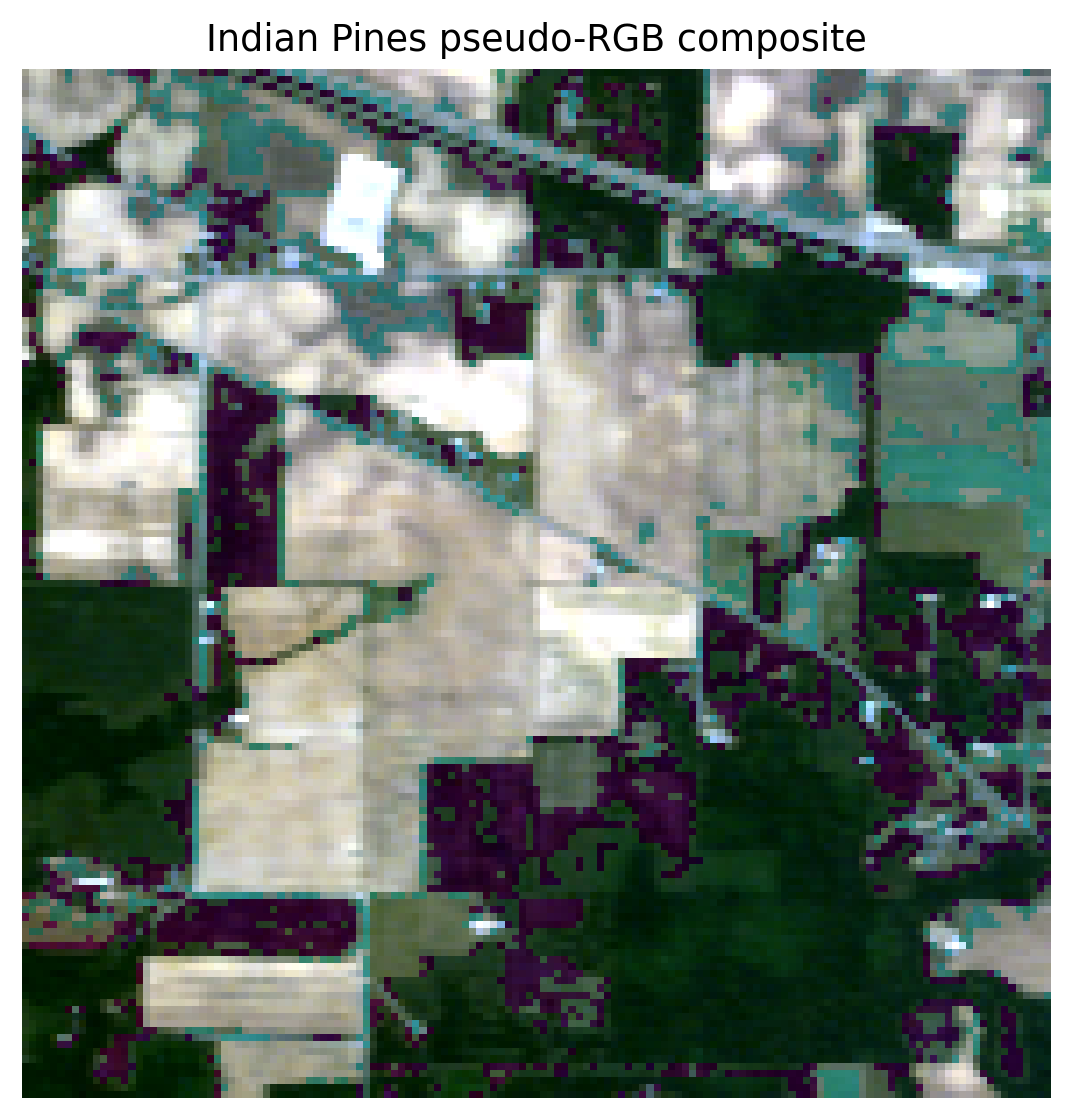
\includegraphics[width=0.62\textwidth]{outputs/figures/01_pseudo_rgb.png}
\caption{Pseudo-RGB visualization of the Indian Pines hyperspectral image.}
\end{figure}

\subsection{Ground-Truth Map}

The ground-truth map shows the spatial position of labeled classes. It is important because the labels are not randomly distributed; neighboring pixels often belong to the same land-cover type. However, for this project, each labeled pixel is treated as an independent instance.

\begin{figure}[H]
\centering
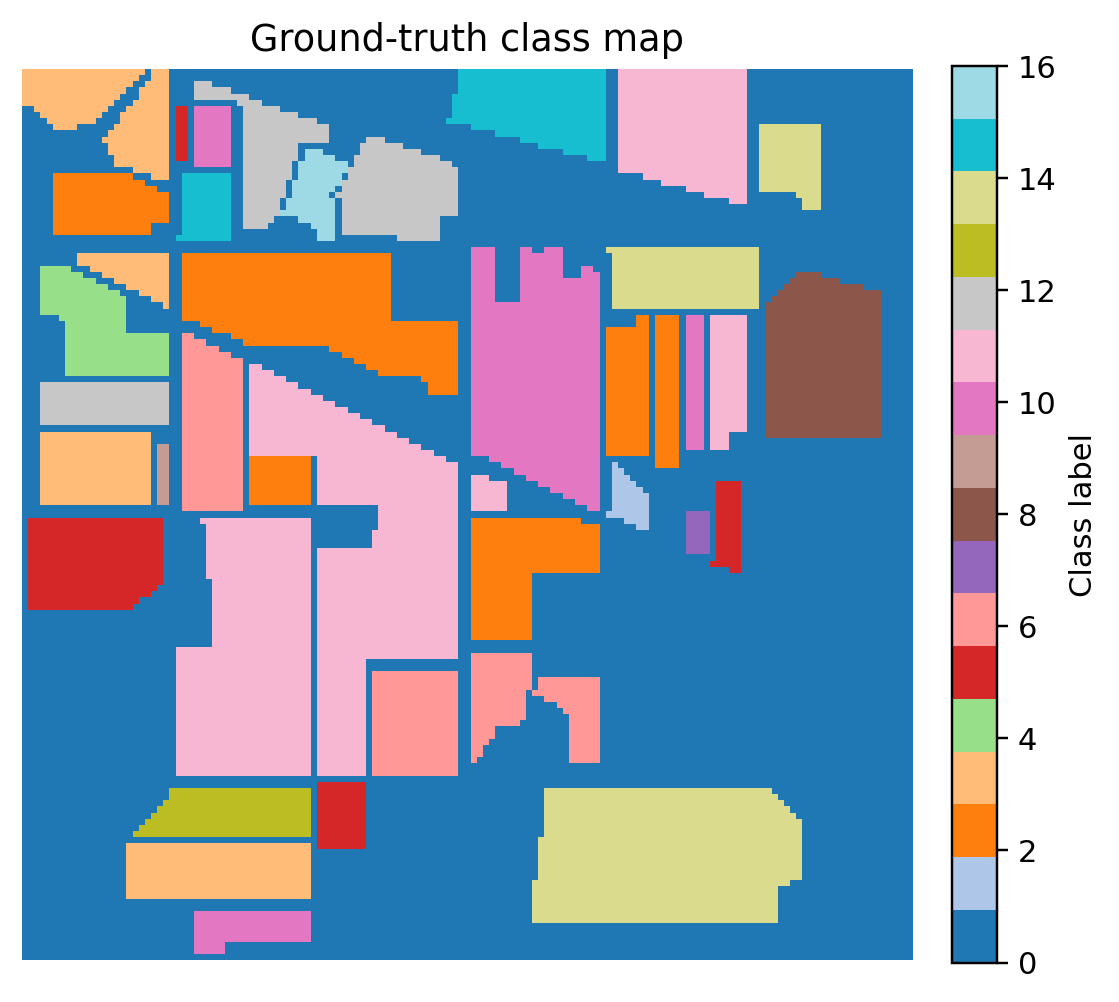
\includegraphics[width=0.62\textwidth]{outputs/figures/02_ground_truth.png}
\caption{Ground-truth map. Label 0 represents unlabeled pixels and labels 1--16 represent land-cover classes.}
\end{figure}

\subsection{Class Imbalance}

The dataset is clearly imbalanced. For example, Soybean-mintill has 2,455 pixels, while Oats has only 20 pixels. This imbalance matters because a classifier can achieve high accuracy by learning the large classes while performing poorly on small classes.

\begin{figure}[H]
\centering
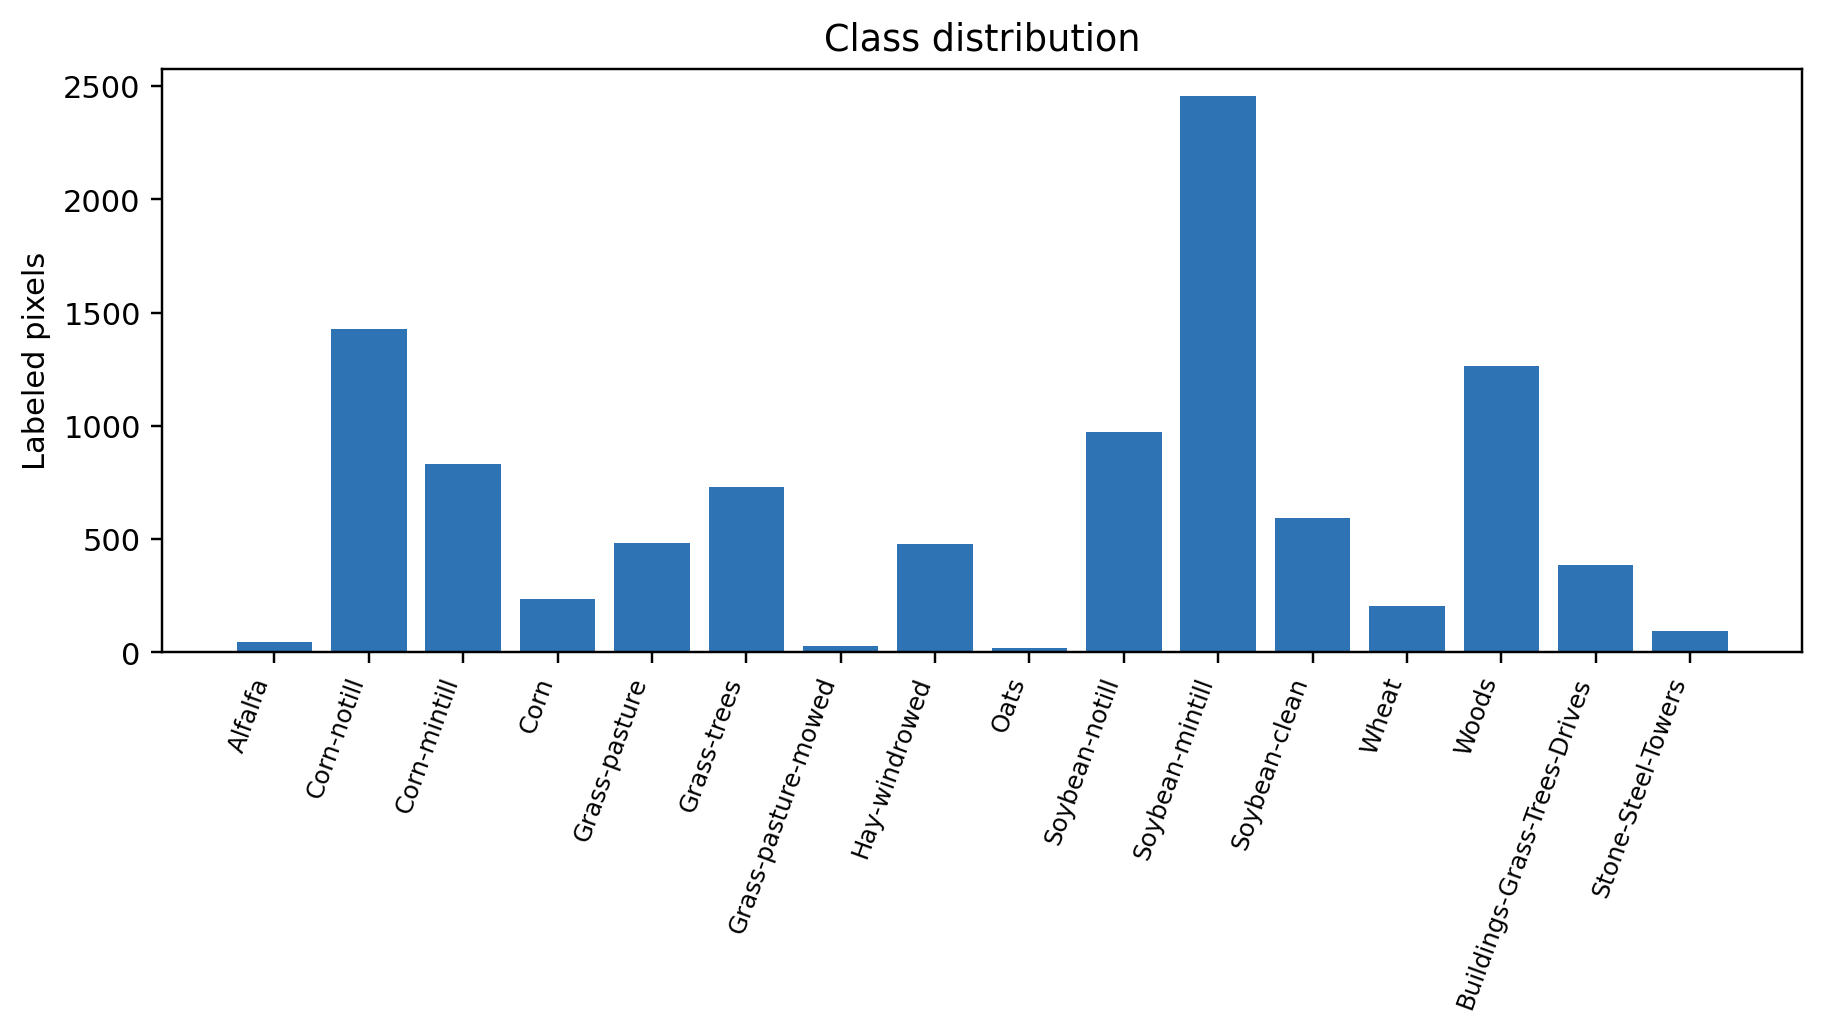
\includegraphics[width=0.95\textwidth]{outputs/figures/03_class_distribution.png}
\caption{Class distribution of labeled pixels.}
\end{figure}

\subsection{Spectral Signature Analysis}

Each class has a spectral signature. A spectral signature is the pattern of reflectance values across the spectral bands. If two classes have clearly different signatures, they are easier to classify. If their signatures are similar, the model may confuse them.

\begin{figure}[H]
\centering
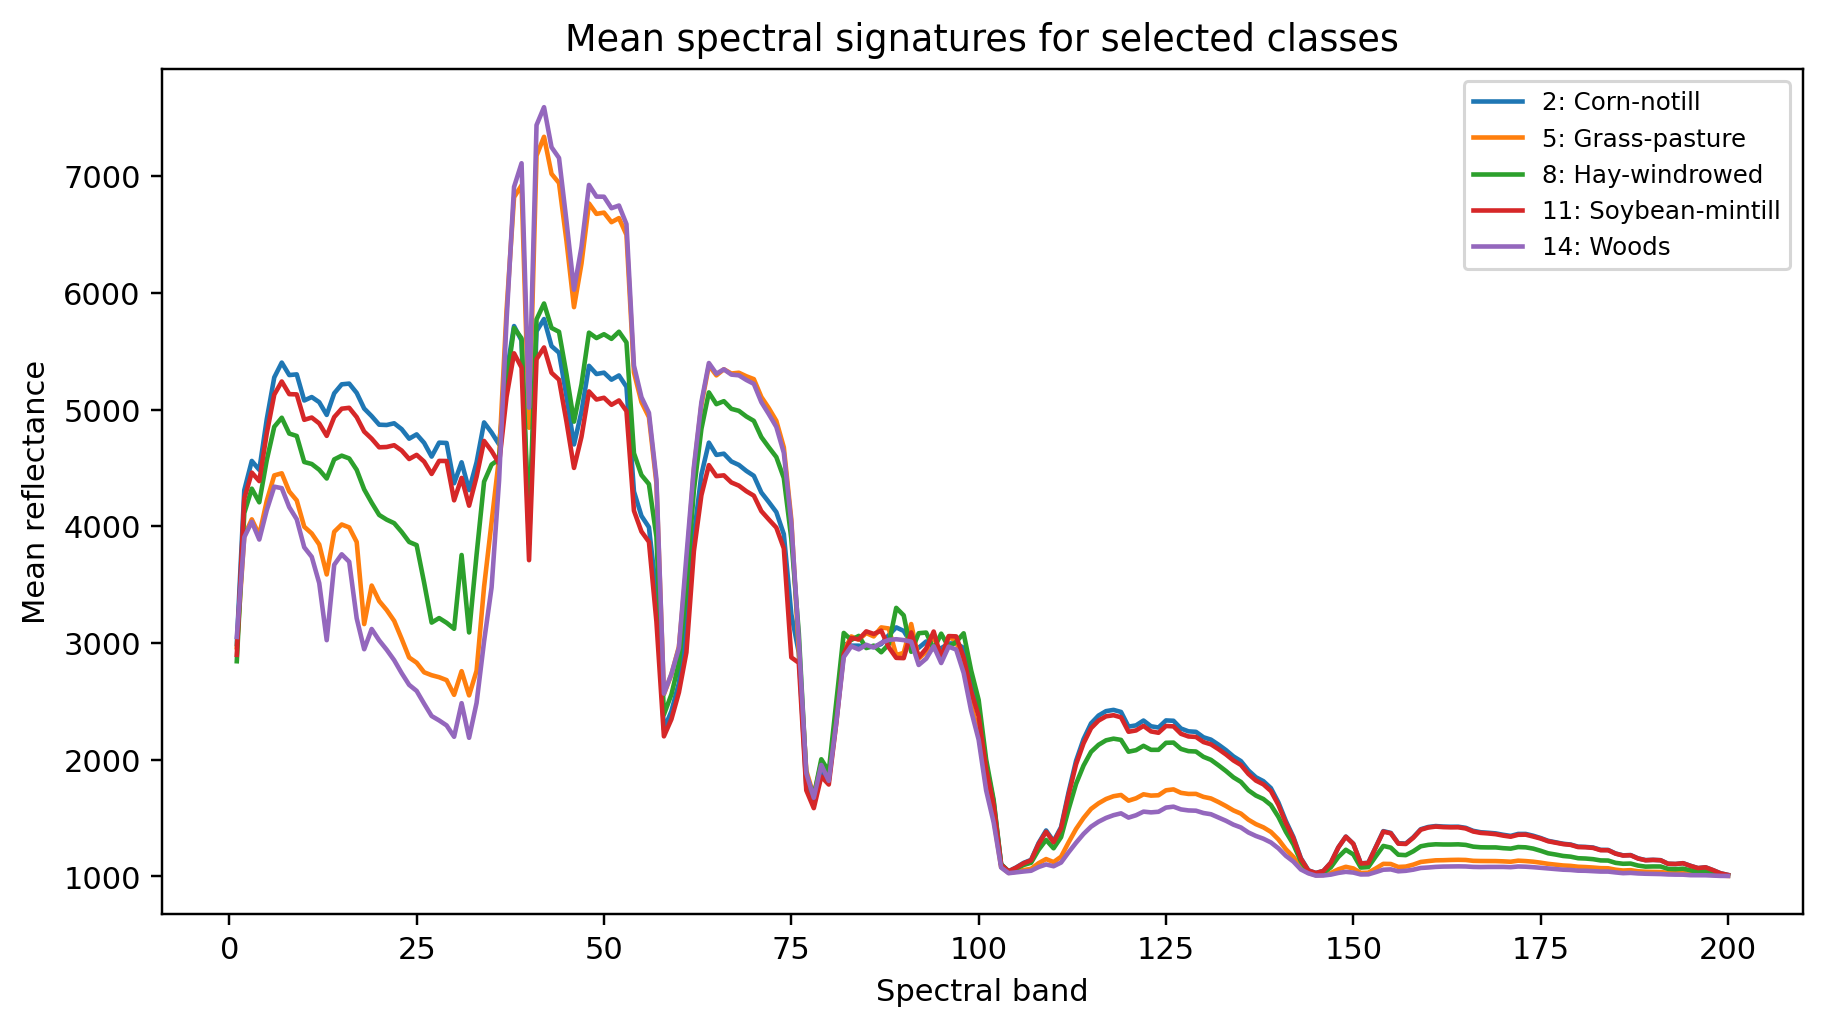
\includegraphics[width=0.82\textwidth]{outputs/figures/04_mean_spectra.png}
\caption{Mean spectral signatures for selected classes.}
\end{figure}

The spectral signature plot shows that different land-cover classes have different average reflectance patterns. This confirms that spectral bands contain useful information for classification.

\subsection{Feature Analysis and Correlation}

The dataset has 200 spectral features. In hyperspectral data, neighboring bands often have strong correlation because adjacent wavelengths measure similar physical properties. A correlation heatmap was used to inspect this relationship.

\begin{figure}[H]
\centering
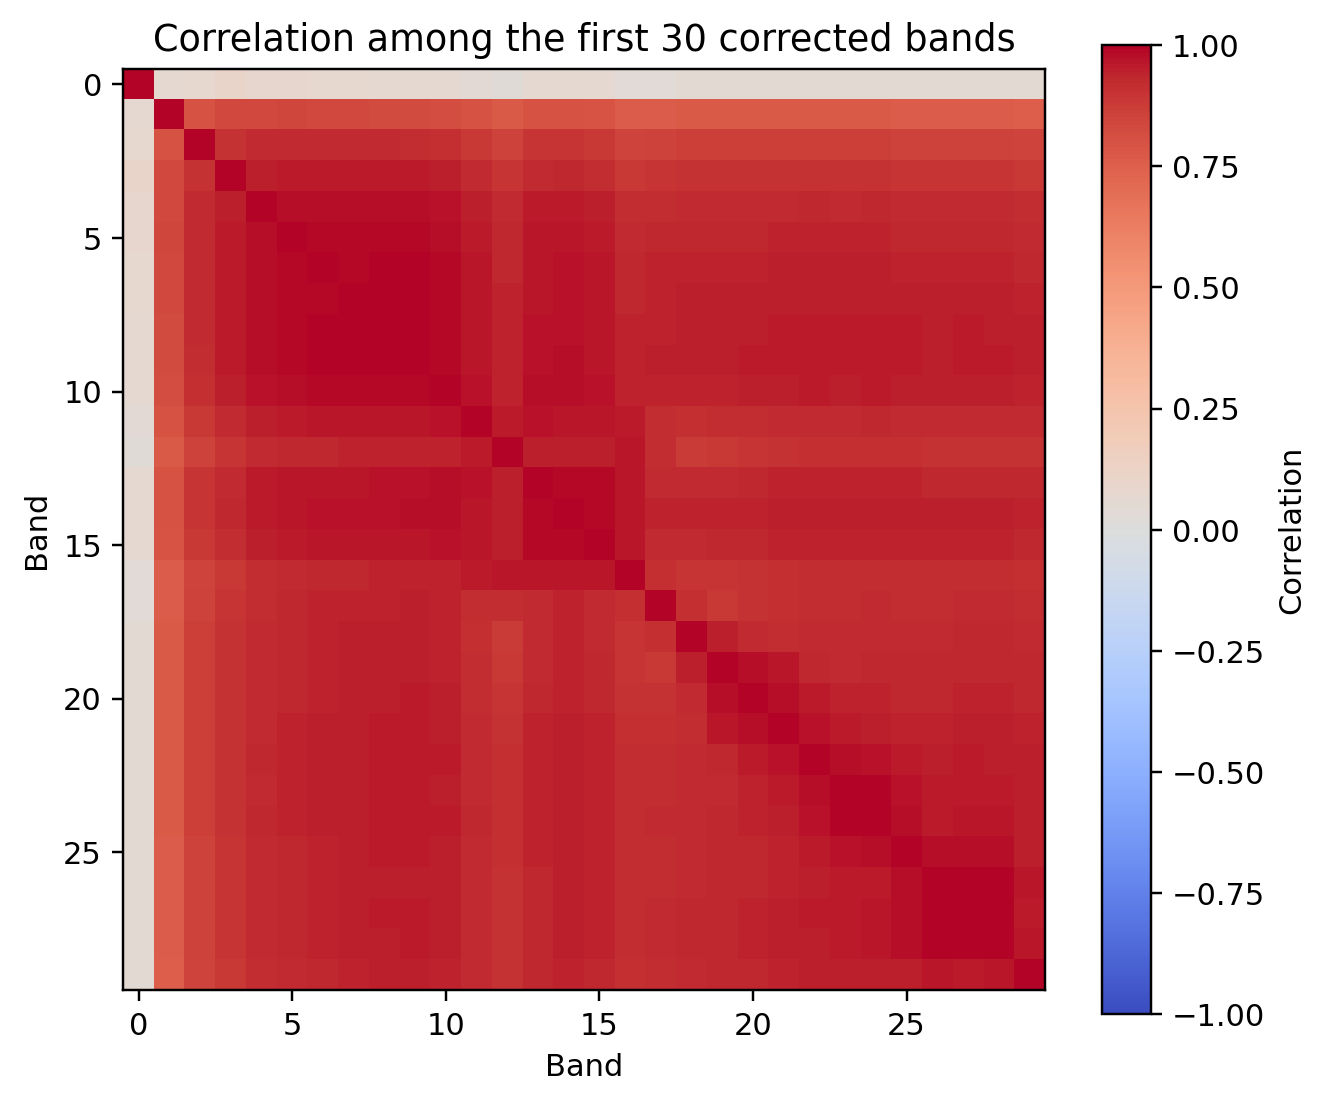
\includegraphics[width=0.72\textwidth]{outputs/figures/05_band_correlation.png}
\caption{Correlation heatmap for the first 30 corrected spectral bands.}
\end{figure}

The heatmap shows strong correlations between many bands. This supports the decision to apply dimensionality reduction. Keeping all 200 bands may increase computation time and may also introduce redundancy.

\subsection{Exploration Code}

The pseudo-RGB image, class distribution, spectral signatures, and correlation heatmap were produced with Python. The following excerpt shows the main exploration operations.

\begin{lstlisting}
import pandas as pd
import matplotlib.pyplot as plt

class_counts = (
    pd.Series(y)
    .value_counts()
    .sort_index()
    .rename_axis("class_id")
    .reset_index(name="pixels")
)

plt.figure(figsize=(12, 5))
plt.bar(class_counts["class_id"], class_counts["pixels"])
plt.xlabel("Class label")
plt.ylabel("Number of pixels")
plt.title("Class Distribution")
plt.show()

corr = np.corrcoef(X[:, :30], rowvar=False)
plt.imshow(corr, cmap="coolwarm", vmin=-1, vmax=1)
plt.colorbar(label="Correlation")
plt.title("Correlation Among First 30 Bands")
plt.show()
\end{lstlisting}

\section{Data Cleaning and Preprocessing}

\subsection{Cleaning Checks}

The cleaning stage checks whether the dataset is suitable for modeling and records the decision made for each issue. The following operations were performed:

\begin{enumerate}
    \item \textbf{Use corrected cube:} The corrected dataset was selected because noisy and water-absorption bands were already removed.
    \item \textbf{Remove unlabeled pixels:} Pixels with label 0 were excluded from modeling because they are not valid land-cover classes.
    \item \textbf{Check missing values:} The feature matrix contains 0 missing values.
    \item \textbf{Check infinite values:} The feature matrix contains 0 infinite values.
    \item \textbf{Check duplicate rows:} No duplicate spectral rows were found among the labeled pixels.
    \item \textbf{Diagnose outliers:} The IQR rule was applied band-by-band to identify unusual spectral values.
\end{enumerate}

\subsection{Missing-Value Filling Method}

Although no missing values were found, a filling method was still defined. The modeling pipelines include \texttt{SimpleImputer(strategy="median")} before scaling and PCA. Median imputation is appropriate for continuous numerical bands because it is more robust to extreme values than mean imputation. The imputer is fitted only on training data inside each pipeline, so test data and validation folds do not leak information into preprocessing.

\subsection{IQR Outlier Diagnostics}

The interquartile range (IQR) rule was used to flag values below $Q1 - 1.5 \times IQR$ or above $Q3 + 1.5 \times IQR$. This method identified 27,593 band-level flags across the feature matrix. There were 91 spectral bands with at least one IQR flag and 2,826 labeled pixels with at least one flagged band. The most frequently flagged band was band 40, with 1,803 flagged pixels.

\begin{figure}[H]
\centering
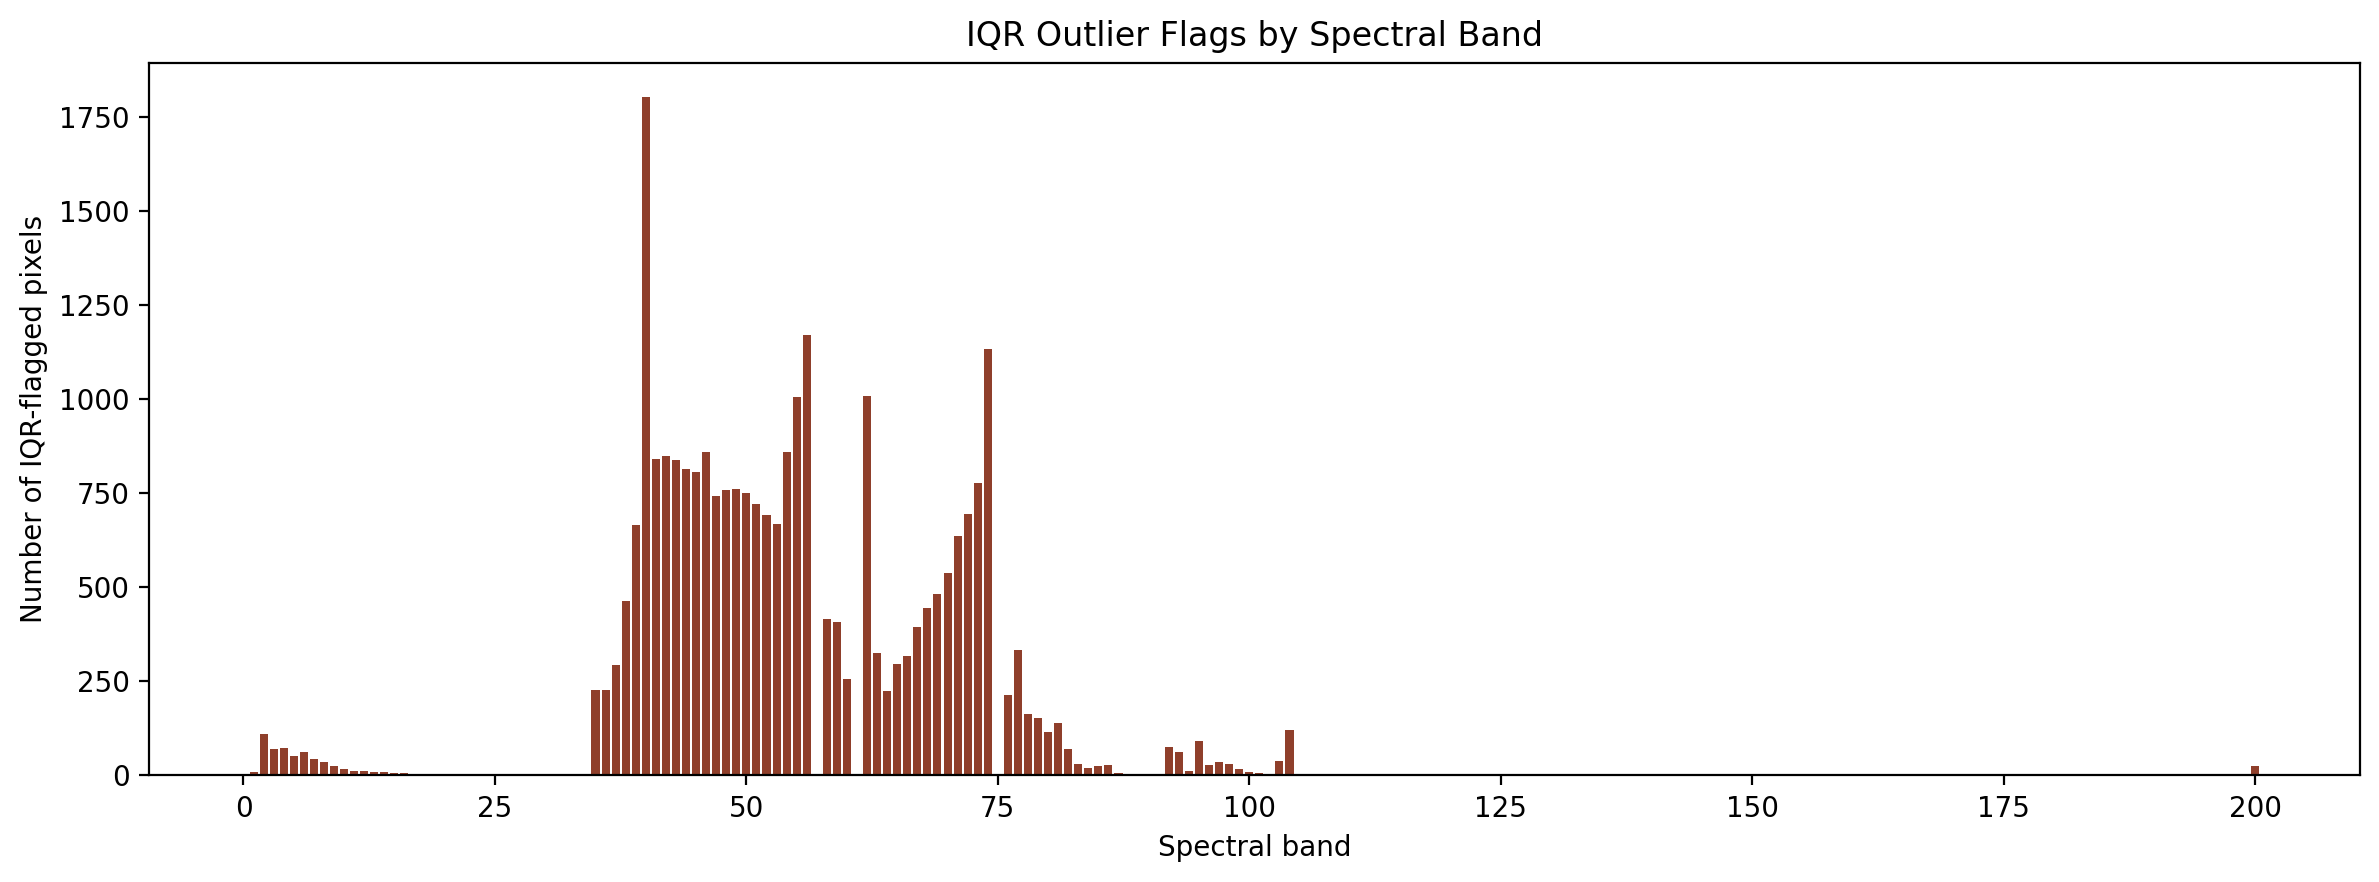
\includegraphics[width=0.92\textwidth]{outputs/figures/07_iqr_outlier_flags_by_band.png}
\caption{IQR outlier flags per spectral band. The flags are used for diagnosis, not automatic deletion.}
\end{figure}

The IQR-flagged pixels were not removed. In hyperspectral data, an unusual reflectance value can be a valid physical signature of a land-cover material, not necessarily an error. Also, several classes are very small, such as Oats with 20 pixels, Grass-pasture-mowed with 28 pixels, and Alfalfa with 46 pixels. Removing IQR-flagged labeled pixels could damage minority-class representation and make the classification problem biased toward majority classes.

\subsection{Band and Pixel Cleaning Visualization}

The reference notebook used band maps, pixel signatures, and pixel heatmaps to make the hyperspectral cube easier to interpret. A similar but deterministic diagnostic was added here for the cleaning stage. It uses band 40, the band with the highest number of IQR flags, and one labeled class-15 pixel that has 67 flagged bands. This makes the cleaning decision more transparent: the flagged values form part of a complete spectral pattern rather than automatically proving that the pixel is invalid.

\begin{figure}[H]
\centering
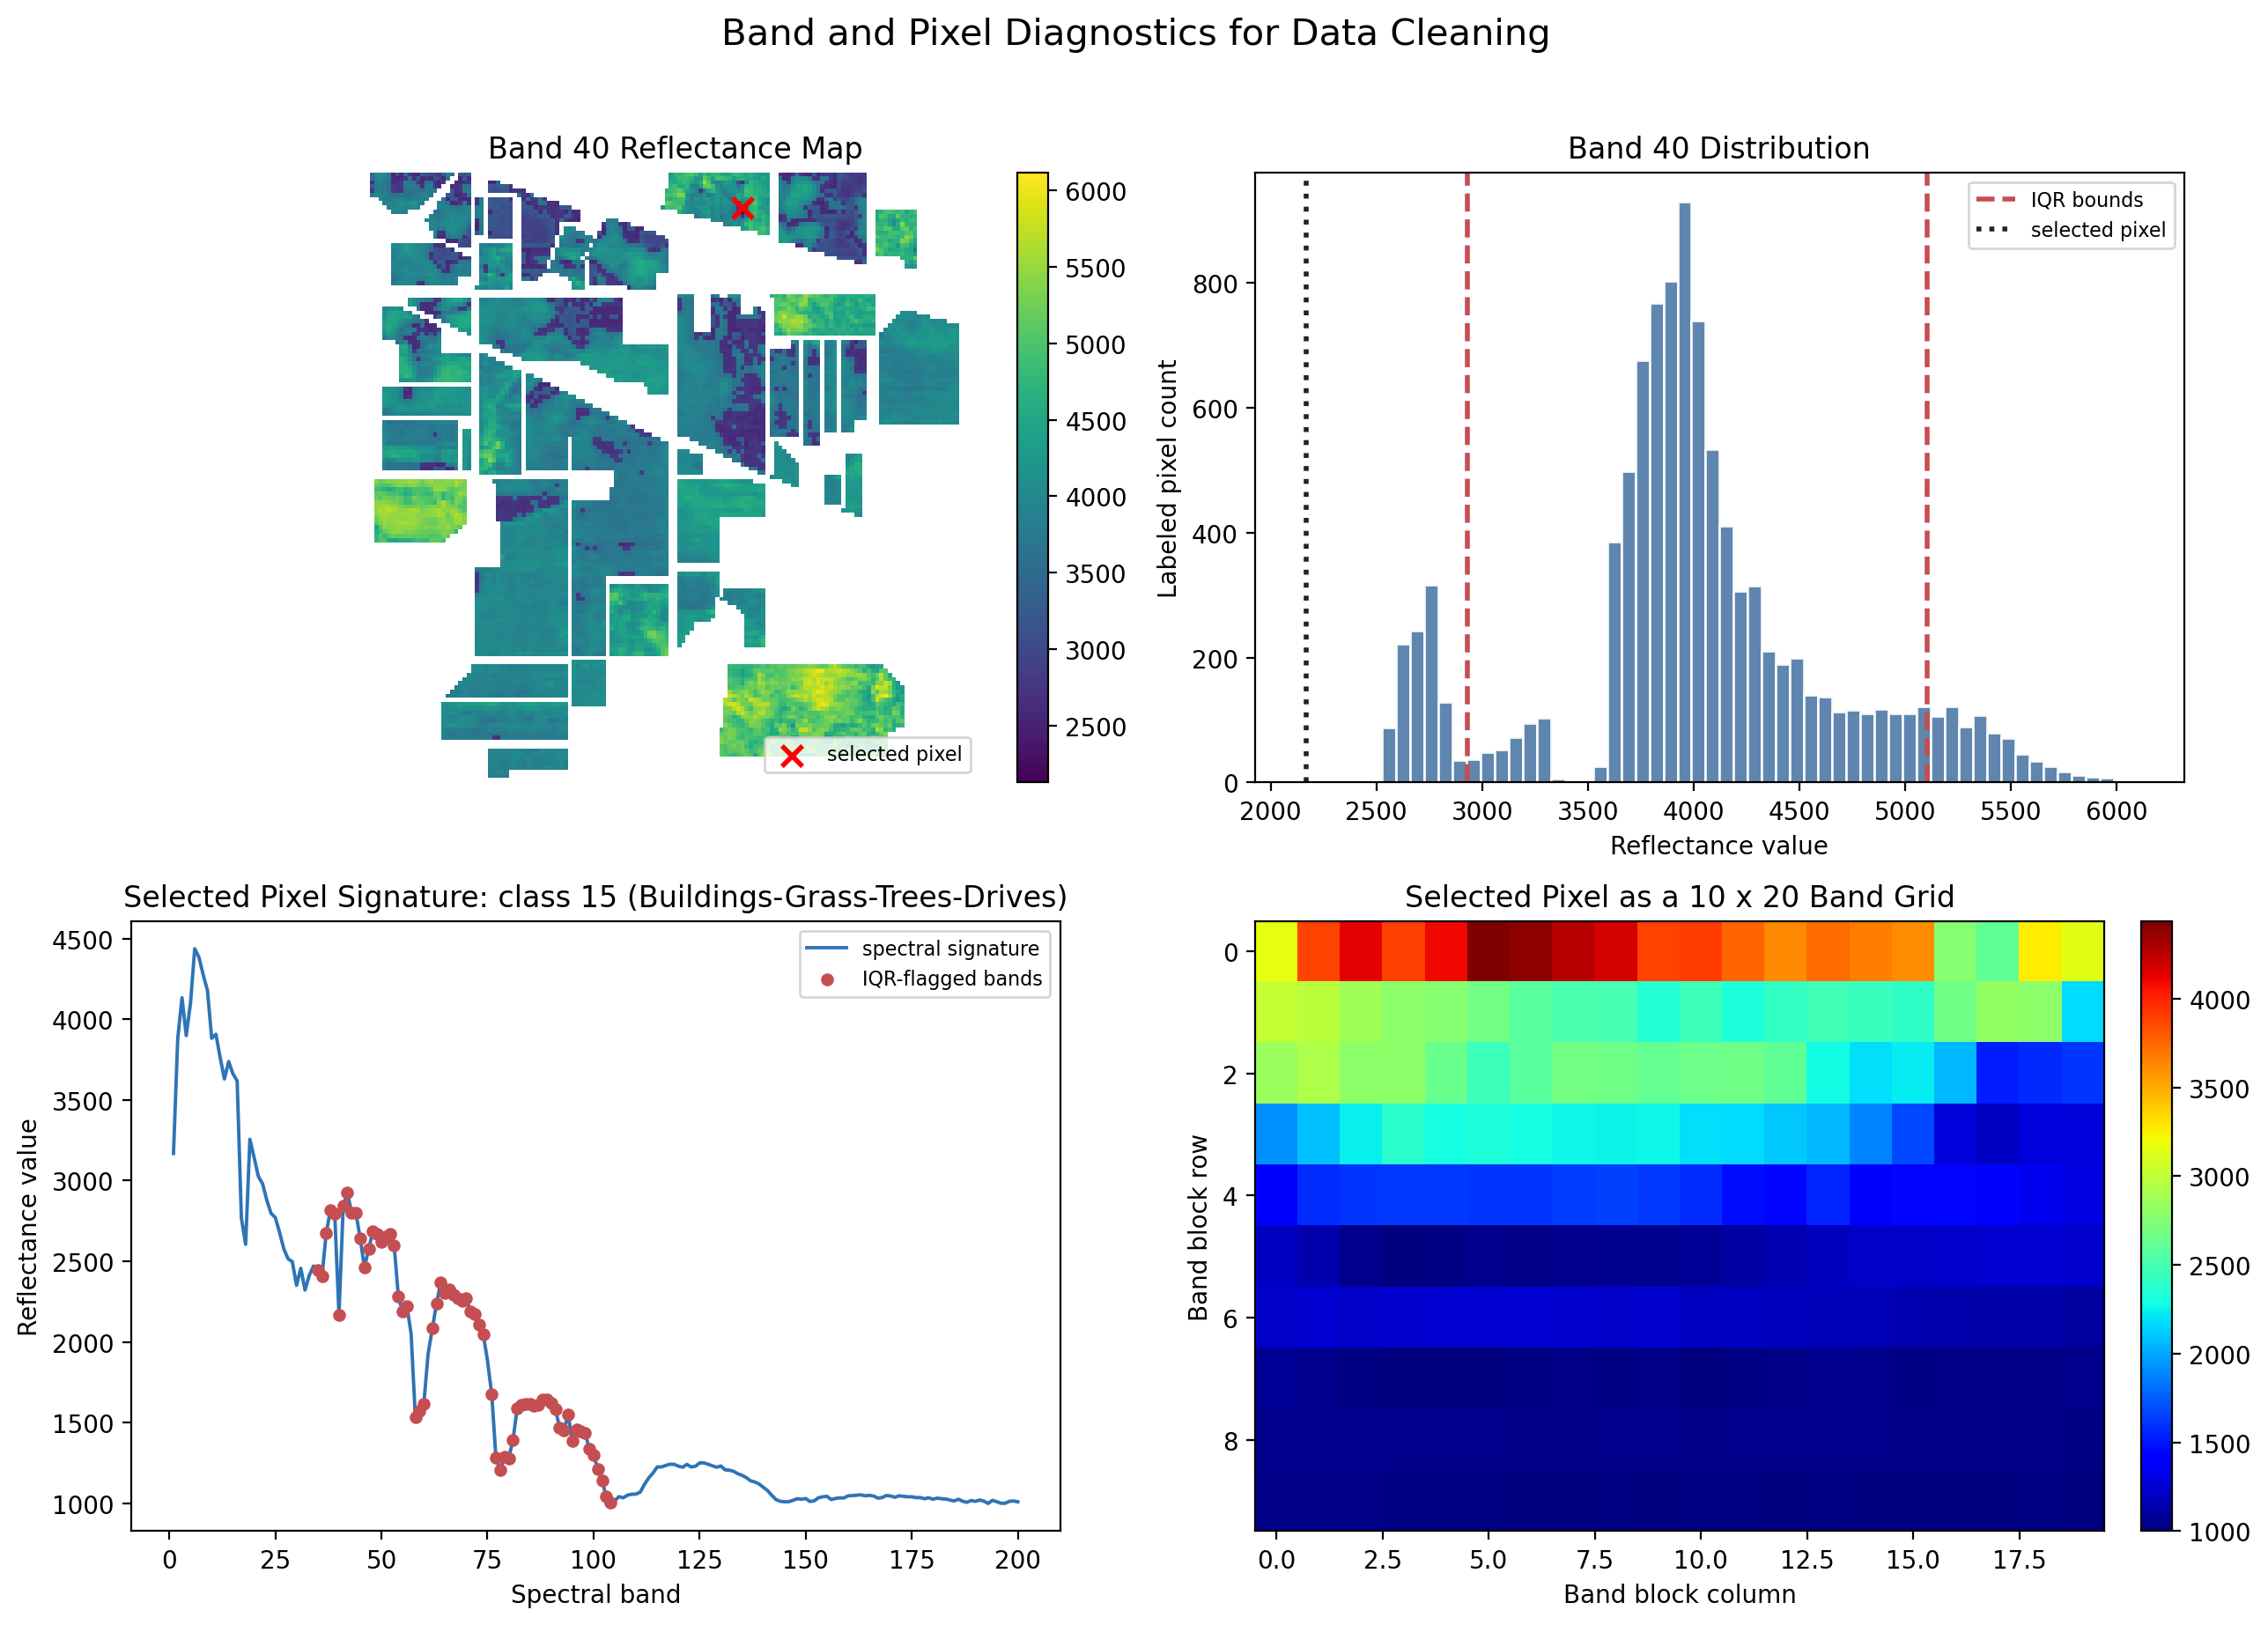
\includegraphics[width=0.96\textwidth]{outputs/figures/08_band_pixel_cleaning_diagnostics.png}
\caption{Band and pixel diagnostics for data cleaning. The figure shows the band-40 reflectance map, band-40 distribution with IQR bounds, the selected pixel's spectral signature, and the selected pixel reshaped as a $10 \times 20$ band grid.}
\end{figure}

\subsection{Encoding Decision}

One-hot encoding was considered but not applied to the input features. The predictors are 200 continuous spectral bands, not categorical variables. One-hot encoding would be appropriate for categorical columns such as sensor type, region name, or soil category, but those variables are not present in this dataset. The target labels are already integer class IDs from 1 to 16, which is the format expected by the scikit-learn classifiers used in this project.

\subsection{Feature Selection and Embedding Rationale}

Traditional feature selection chooses a subset of original features. In this project, PCA was chosen instead because hyperspectral bands are continuous and highly correlated. PCA does not simply remove bands; it creates new uncorrelated components that summarize the original bands. Therefore, PCA acts as the project's feature embedding method by converting each 200-band pixel vector into a 20-dimensional representation.

\subsection{Standardization}

Standardization was applied before PCA and model training. For each feature, standardization transforms the values as:

\[
z = \frac{x - \mu}{\sigma}
\]

where $x$ is the original value, $\mu$ is the mean, and $\sigma$ is the standard deviation. This step is important because PCA, KNN, and SVM are sensitive to feature scale.

\subsection{Train-Test Split Code}

A stratified split was used so that each class keeps a similar proportion in the training and test sets.

\begin{lstlisting}
from sklearn.model_selection import train_test_split

RANDOM_STATE = 42
TEST_SIZE = 0.20

X_train, X_test, y_train, y_test = train_test_split(
    X,
    y,
    test_size=TEST_SIZE,
    random_state=RANDOM_STATE,
    stratify=y
)
\end{lstlisting}

\section{Dimensionality Reduction with PCA}

\subsection{Why PCA Was Used}

Principal Component Analysis was used for dimensionality reduction. The original dataset has 200 spectral features. Because many bands are correlated, PCA can reduce the number of features while preserving the main information.

The benefits of PCA in this project are:

\begin{itemize}
    \item It reduces the feature space from 200 dimensions to 20 dimensions.
    \item It removes some redundant information.
    \item It makes model training faster.
    \item It helps reduce noise.
    \item It creates uncorrelated principal components.
\end{itemize}

\subsection{PCA Explained Variance}

The cumulative explained variance curve shows how much information is preserved as the number of principal components increases.

\begin{figure}[H]
\centering
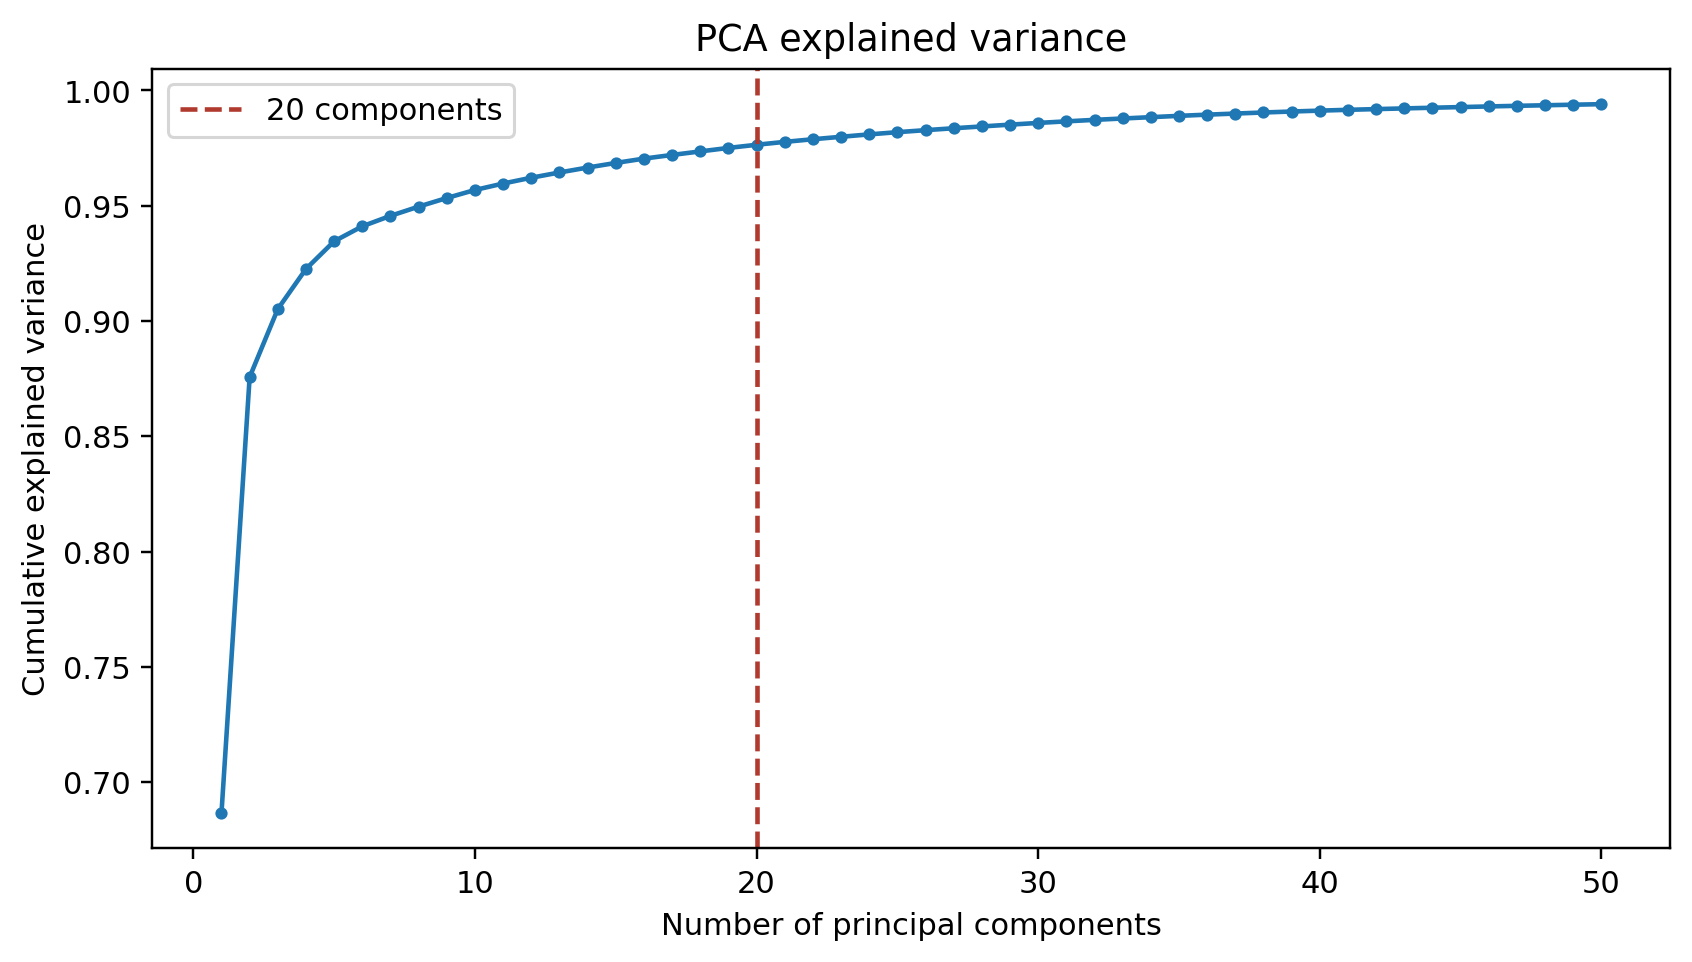
\includegraphics[width=0.85\textwidth]{outputs/figures/10_pca_explained_variance.png}
\caption{Cumulative explained variance from PCA.}
\end{figure}

In the experiments, 20 principal components were used. This value provides a balance between reducing dimensionality and preserving useful information; the first 20 components preserve approximately 97.64\% of the standardized spectral variance.

\subsection{PCA Code}

PCA was applied inside the machine learning pipeline to prevent data leakage. The following code was also used to inspect cumulative explained variance.

\begin{lstlisting}
from sklearn.preprocessing import StandardScaler
from sklearn.decomposition import PCA
from sklearn.impute import SimpleImputer
from sklearn.pipeline import Pipeline

N_COMPONENTS = 20

preprocess_probe = Pipeline([
    ("imputer", SimpleImputer(strategy="median")),
    ("scaler", StandardScaler()),
])

X_preprocessed = preprocess_probe.fit_transform(X)

pca_probe = PCA(n_components=50, random_state=42)
pca_probe.fit(X_preprocessed)

cum_var = np.cumsum(pca_probe.explained_variance_ratio_)
print(cum_var[N_COMPONENTS - 1])
\end{lstlisting}

\section{Machine Learning Algorithms}

\subsection{Baseline Algorithms}

Two baselines were included:

\begin{itemize}
    \item \textbf{Most Common Class baseline:} This classifier always predicts the majority class. It is useful because it shows the minimum performance that a real model should beat.
    \item \textbf{k-Nearest Neighbors:} KNN was used as a stronger baseline. It predicts a class based on the labels of nearby samples in feature space.
\end{itemize}

\subsection{Main Algorithms}

Three main classifiers were selected:

\subsubsection{Random Forest}

Random Forest is an ensemble of decision trees. Each tree is trained on a random subset of data and features, and the final prediction is based on voting. It was selected because:

\begin{itemize}
    \item It handles nonlinear relationships.
    \item It is less likely to overfit than a single decision tree.
    \item It works well on many classification problems.
    \item It can handle complex class boundaries.
\end{itemize}

\subsubsection{Gradient Boosting}

Gradient Boosting builds trees sequentially. Each new tree attempts to correct errors made by previous trees. It was selected because:

\begin{itemize}
    \item It can produce strong predictive performance.
    \item It learns complex patterns step by step.
    \item It is useful when weak learners can be combined into a strong model.
\end{itemize}

\subsubsection{Support Vector Machine}

Support Vector Machine attempts to find a decision boundary that separates classes with a maximum margin. The RBF kernel was used to allow nonlinear decision boundaries. SVM was selected because:

\begin{itemize}
    \item It performs well in high-dimensional spaces.
    \item It is suitable for spectral classification problems.
    \item It works effectively after standardization and PCA.
    \item The RBF kernel can model nonlinear class separation.
\end{itemize}

\section{Experimental Design}

\subsection{Train-Test Split}

The dataset was split into training and testing sets:

\begin{itemize}
    \item 80\% of labeled pixels were used for training.
    \item 20\% of labeled pixels were used for testing.
    \item Stratified splitting was used to keep class proportions similar in both sets.
\end{itemize}

Stratification is important because the dataset is imbalanced. Without stratification, small classes could be underrepresented or missing from the test set.

\subsection{Pipeline Design}

For KNN, Random Forest, Gradient Boosting, and SVM, the following pipeline was used:

\[
\text{SimpleImputer} \rightarrow \text{StandardScaler} \rightarrow \text{PCA} \rightarrow \text{Classifier}
\]

Using a pipeline prevents data leakage because filling, scaling, and PCA are fitted only on the training data during each training or cross-validation step.

\subsection{Model Definition Code}

The following code shows the baseline models and the three main classifiers used in the experiments.

\begin{lstlisting}
from sklearn.dummy import DummyClassifier
from sklearn.decomposition import PCA
from sklearn.neighbors import KNeighborsClassifier
from sklearn.ensemble import RandomForestClassifier, GradientBoostingClassifier
from sklearn.impute import SimpleImputer
from sklearn.svm import SVC
from sklearn.pipeline import Pipeline
from sklearn.preprocessing import StandardScaler

models = {
    "Most Common Class": DummyClassifier(strategy="most_frequent"),

    "k-Nearest Neighbors": Pipeline([
        ("imputer", SimpleImputer(strategy="median")),
        ("scaler", StandardScaler()),
        ("pca", PCA(n_components=20, random_state=42)),
        ("model", KNeighborsClassifier(n_neighbors=5)),
    ]),

    "Random Forest": Pipeline([
        ("imputer", SimpleImputer(strategy="median")),
        ("scaler", StandardScaler()),
        ("pca", PCA(n_components=20, random_state=42)),
        ("model", RandomForestClassifier(
            n_estimators=80,
            class_weight="balanced",
            random_state=42,
            n_jobs=1
        )),
    ]),

    "Gradient Boosting": Pipeline([
        ("imputer", SimpleImputer(strategy="median")),
        ("scaler", StandardScaler()),
        ("pca", PCA(n_components=20, random_state=42)),
        ("model", GradientBoostingClassifier(
            n_estimators=45,
            learning_rate=0.10,
            max_depth=3,
            random_state=42
        )),
    ]),

    "Support Vector Machine": Pipeline([
        ("imputer", SimpleImputer(strategy="median")),
        ("scaler", StandardScaler()),
        ("pca", PCA(n_components=20, random_state=42)),
        ("model", SVC(
            kernel="rbf",
            C=10,
            gamma="scale",
            class_weight="balanced"
        )),
    ]),
}
\end{lstlisting}

\subsection{Evaluation Metrics}

Several metrics were used because accuracy alone can be misleading for imbalanced datasets.

\begin{itemize}
    \item \textbf{Accuracy:} Measures the overall proportion of correct predictions.
    \item \textbf{Precision:} Measures how many predicted samples of a class are actually correct.
    \item \textbf{Recall:} Measures how many actual samples of a class are correctly found.
    \item \textbf{F1-score:} Harmonic mean of precision and recall.
    \item \textbf{Macro F1-score:} Average F1-score across all classes, treating each class equally.
    \item \textbf{Weighted F1-score:} Average F1-score weighted by the number of samples in each class.
    \item \textbf{Confusion matrix:} Shows class-wise prediction errors.
    \item \textbf{Cross-validation accuracy:} Estimates generalization performance across multiple folds.
\end{itemize}

The F1-score is especially important because the dataset is imbalanced. Macro F1 gives more visibility to minority classes, while weighted F1 reflects performance according to the dataset distribution.

\subsection{Training and Evaluation Code}

Each model was trained on the training set and evaluated on the test set using accuracy, F1-scores, classification report, and confusion matrix.

\begin{lstlisting}
from sklearn.metrics import (
    accuracy_score,
    classification_report,
    confusion_matrix
)

results = {}

for name, model in models.items():
    model.fit(X_train, y_train)
    y_pred = model.predict(X_test)

    report = classification_report(
        y_test,
        y_pred,
        output_dict=True,
        zero_division=0
    )

    results[name] = {
        "accuracy": accuracy_score(y_test, y_pred),
        "macro_f1": report["macro avg"]["f1-score"],
        "weighted_f1": report["weighted avg"]["f1-score"],
        "confusion_matrix": confusion_matrix(y_test, y_pred)
    }
\end{lstlisting}

\subsection{Cross-Validation Setup}

A 3-fold stratified cross-validation strategy was used. The data were divided into three folds while preserving class proportions. Each model was trained and validated three times, and the average accuracy was reported. Because preprocessing is inside the pipeline, the imputer, scaler, and PCA transformation are refit inside each fold instead of being learned from the full dataset.

\subsection{Cross-Validation Code}

\begin{lstlisting}
from sklearn.model_selection import StratifiedKFold, cross_val_score

cv = StratifiedKFold(
    n_splits=3,
    shuffle=True,
    random_state=42
)

for name, model in models.items():
    scores = cross_val_score(
        model,
        X,
        y,
        cv=cv,
        scoring="accuracy",
        n_jobs=1
    )
    print(name, scores.mean(), scores.std())
\end{lstlisting}

\subsection{Hyperparameter Tuning Setup}

Random Forest was tuned using two methods:

\begin{itemize}
    \item \textbf{RandomizedSearchCV:} Randomly tests parameter combinations. It is faster than grid search when the search space is large.
    \item \textbf{GridSearchCV:} Tests all parameter combinations in a smaller predefined grid.
\end{itemize}

The tuned parameters included:

\begin{itemize}
    \item Number of trees.
    \item Maximum depth.
    \item Minimum samples required to split a node.
    \item Minimum samples required at a leaf node.
\end{itemize}

\subsection{Hyperparameter Tuning Code}

The following code shows the Random Forest tuning setup. The grid was intentionally kept moderate so the experiment could run in a reasonable amount of time.

\begin{lstlisting}
from sklearn.decomposition import PCA
from sklearn.ensemble import RandomForestClassifier
from sklearn.impute import SimpleImputer
from sklearn.model_selection import RandomizedSearchCV, GridSearchCV
from sklearn.pipeline import Pipeline
from sklearn.preprocessing import StandardScaler

rf_pipeline = Pipeline([
    ("imputer", SimpleImputer(strategy="median")),
    ("scaler", StandardScaler()),
    ("pca", PCA(n_components=20, random_state=42)),
    ("model", RandomForestClassifier(
        class_weight="balanced",
        random_state=42,
        n_jobs=1
    )),
])

random_param_dist = {
    "model__n_estimators": [60, 80, 120],
    "model__max_depth": [8, 12, None],
    "model__min_samples_split": [2, 5],
    "model__min_samples_leaf": [1, 2],
}

random_search = RandomizedSearchCV(
    rf_pipeline,
    random_param_dist,
    n_iter=6,
    scoring="accuracy",
    cv=2,
    random_state=42,
    n_jobs=1
)

random_search.fit(X_train, y_train)

grid_param = {
    "model__n_estimators": [80, 120],
    "model__max_depth": [12, None],
    "model__min_samples_split": [2, 5],
    "model__min_samples_leaf": [1],
}

grid_search = GridSearchCV(
    rf_pipeline,
    grid_param,
    scoring="accuracy",
    cv=2,
    n_jobs=1
)

grid_search.fit(X_train, y_train)
\end{lstlisting}

\section{Results and Analysis}

\subsection{Overall Model Comparison}

\begin{table}[H]
\centering
\begin{tabular}{lcccc}
\toprule
\textbf{Model} & \textbf{Test Accuracy} & \textbf{3-Fold CV} & \textbf{Macro F1} & \textbf{Weighted F1} \\
\midrule
Most Common Class & 0.240 & 0.240 $\pm$ 0.000 & 0.024 & 0.093 \\
k-Nearest Neighbors & 0.749 & 0.742 $\pm$ 0.011 & 0.715 & 0.740 \\
Random Forest & 0.794 & 0.778 $\pm$ 0.007 & 0.749 & 0.786 \\
Gradient Boosting & 0.757 & 0.737 $\pm$ 0.006 & 0.682 & 0.750 \\
Support Vector Machine & \textbf{0.812} & \textbf{0.804 $\pm$ 0.007} & \textbf{0.840} & \textbf{0.813} \\
\bottomrule
\end{tabular}
\caption{Model comparison including baselines.}
\end{table}

\subsection{Interpretation of Baselines}

The Most Common Class baseline achieved 23.95\% test accuracy. This is because it always predicts the majority class, which is Soybean-mintill. Its macro F1-score is very low because it completely ignores minority classes.

The k-Nearest Neighbors baseline achieved 74.88\% test accuracy. This is much better than the most-common-class baseline, showing that the spectral features contain strong class information. However, KNN is still weaker than Random Forest and SVM.

\subsection{Interpretation of Main Models}

Random Forest achieved 79.41\% test accuracy. This result shows that ensemble trees can learn useful nonlinear relationships from PCA features.

Gradient Boosting achieved 75.71\% test accuracy. Although boosting is often powerful, in this experiment it performed worse than Random Forest and SVM. A possible reason is that the selected lightweight configuration was chosen to keep computation manageable.

Support Vector Machine achieved the best performance with 81.17\% test accuracy, 80.45\% cross-validation accuracy, and 84.03\% macro F1-score. The high macro F1-score suggests that SVM handled minority classes better than the other tested models.

\begin{figure}[H]
\centering
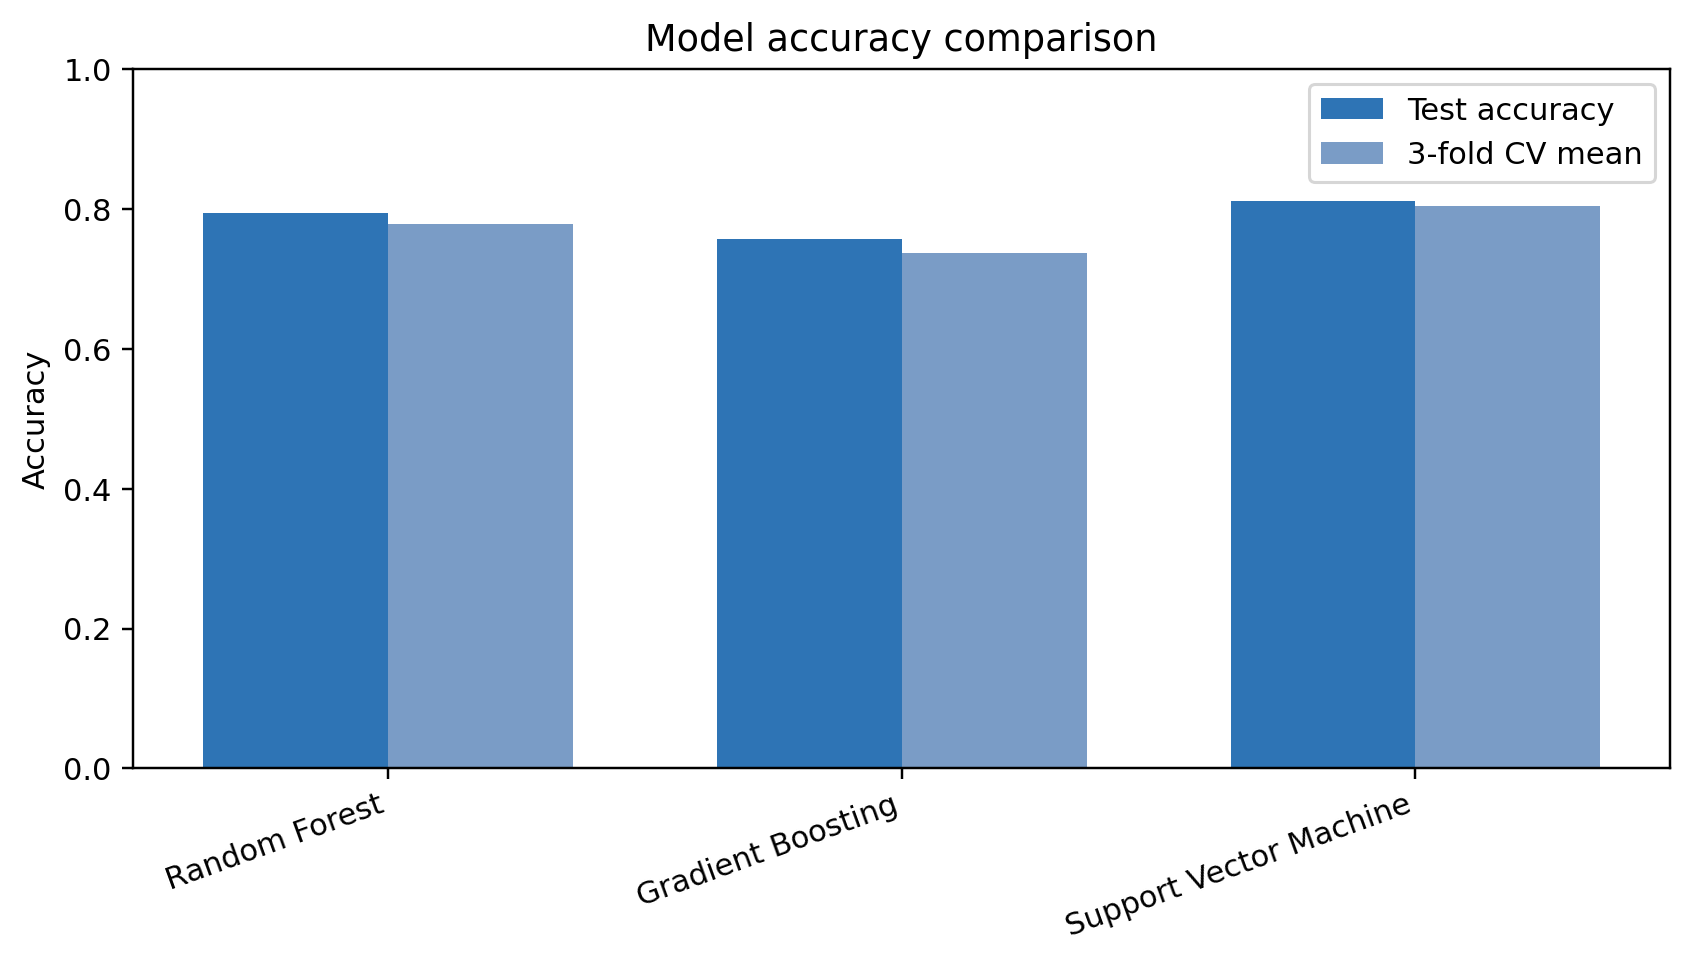
\includegraphics[width=0.85\textwidth]{outputs/figures/09_accuracy_comparison.png}
\caption{Accuracy comparison including baseline models and main classifiers.}
\end{figure}

\section{Confusion Matrix Analysis}

Confusion matrices provide more detailed insight than accuracy alone. In each matrix, the diagonal values represent correct predictions, and off-diagonal values represent errors.

\subsection{Support Vector Machine}

\begin{figure}[H]
\centering
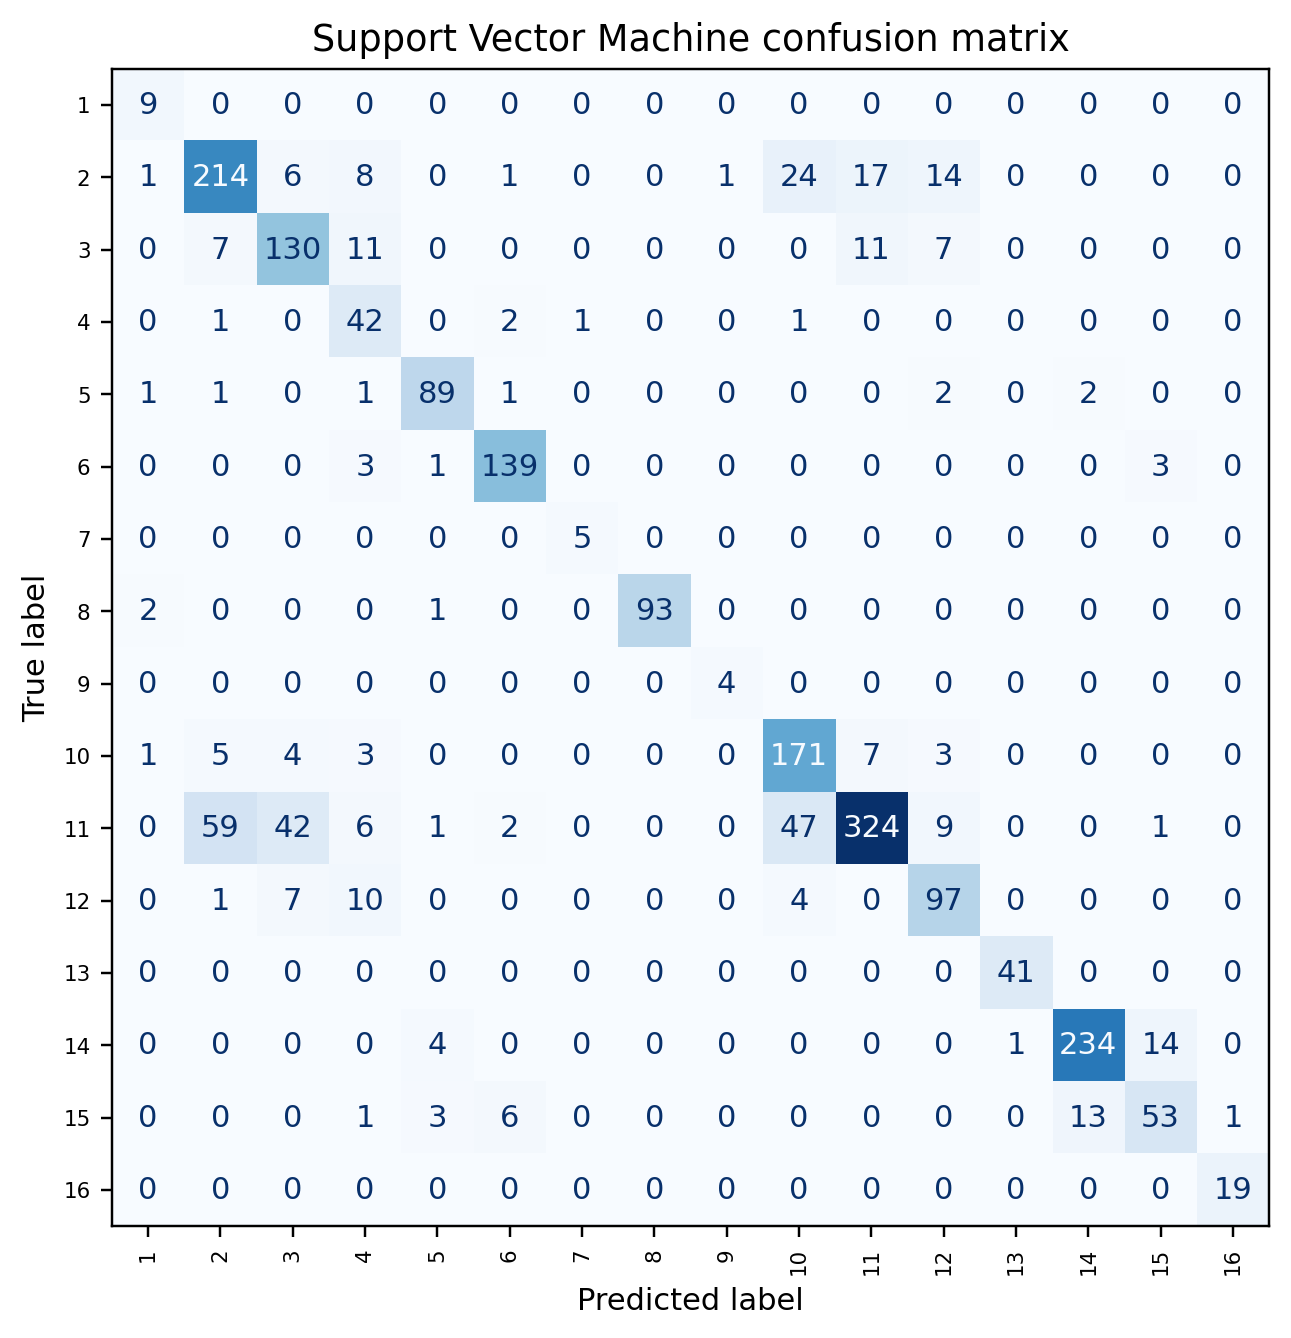
\includegraphics[width=0.78\textwidth]{outputs/figures/06_cm_support_vector_machine.png}
\caption{Confusion matrix for Support Vector Machine.}
\end{figure}

The SVM confusion matrix shows strong diagonal values for many classes, meaning that the model correctly identifies many land-cover categories. Some confusion remains between similar agricultural classes, especially different corn and soybean categories.

\subsection{Random Forest}

\begin{figure}[H]
\centering
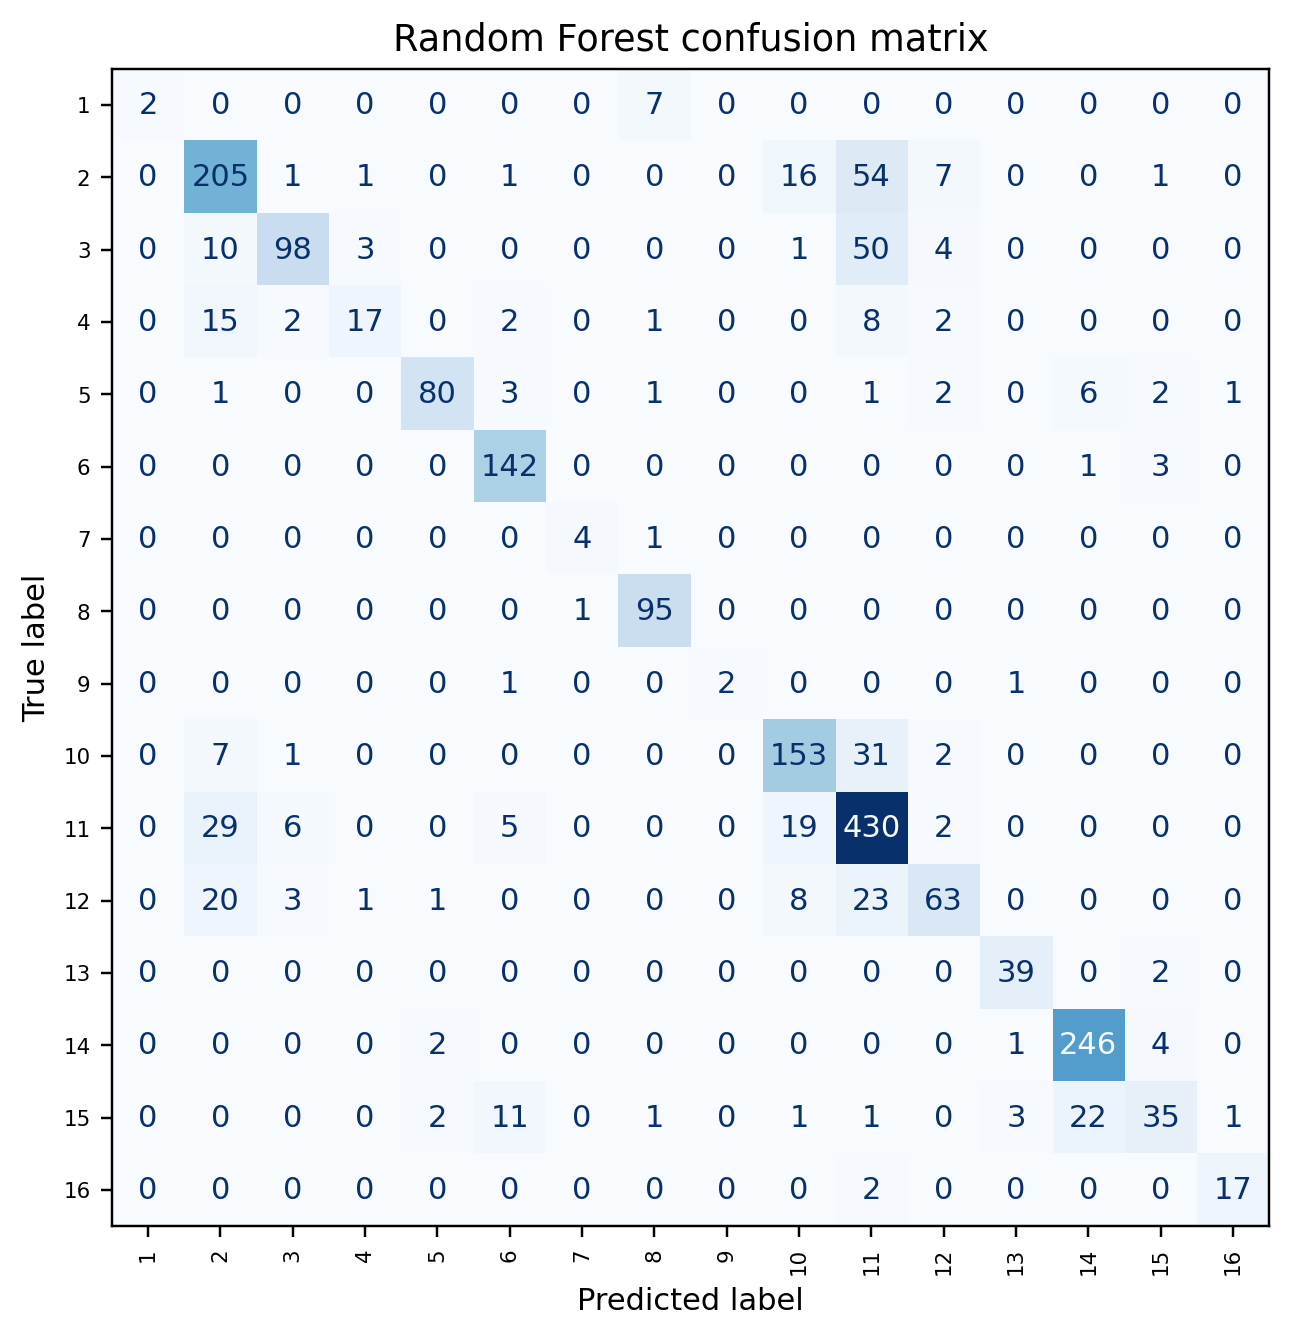
\includegraphics[width=0.78\textwidth]{outputs/figures/06_cm_random_forest.png}
\caption{Confusion matrix for Random Forest.}
\end{figure}

Random Forest performs well overall, but it is slightly weaker than SVM. Its errors are also mainly concentrated among spectrally similar crop classes.

\subsection{Gradient Boosting}

\begin{figure}[H]
\centering
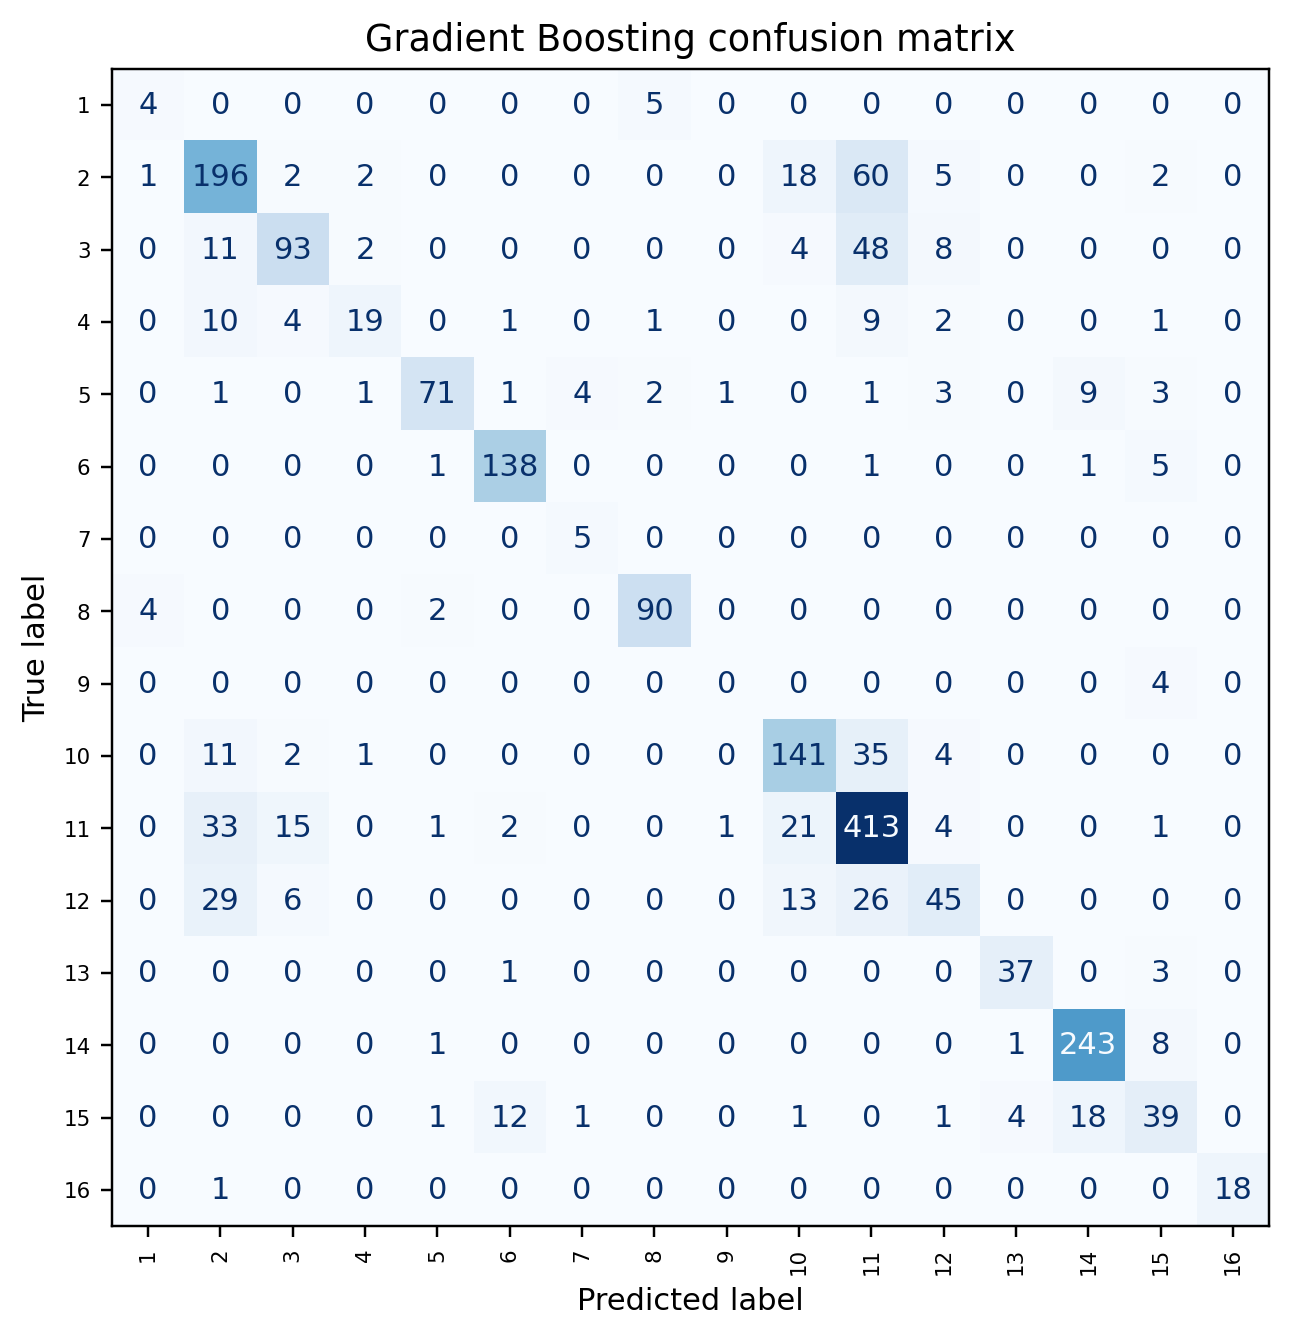
\includegraphics[width=0.78\textwidth]{outputs/figures/06_cm_gradient_boosting.png}
\caption{Confusion matrix for Gradient Boosting.}
\end{figure}

Gradient Boosting gives reasonable results but does not outperform the other main models. With more extensive tuning, it could potentially improve, but the current configuration is less effective than SVM and Random Forest.

\section{Hyperparameter Tuning Results}

Hyperparameter tuning was performed on Random Forest. The tuned Random Forest reached approximately 80.05\% test accuracy. This is slightly higher than the untuned Random Forest result of 79.41\%, meaning the original Random Forest configuration was already reasonable, but tuning still provided a small improvement.

The tuning process is still useful because it demonstrates how model parameters affect performance. In a larger project, a wider search space and more cross-validation folds could be used, but this would require more computation time.

\begin{figure}[H]
\centering
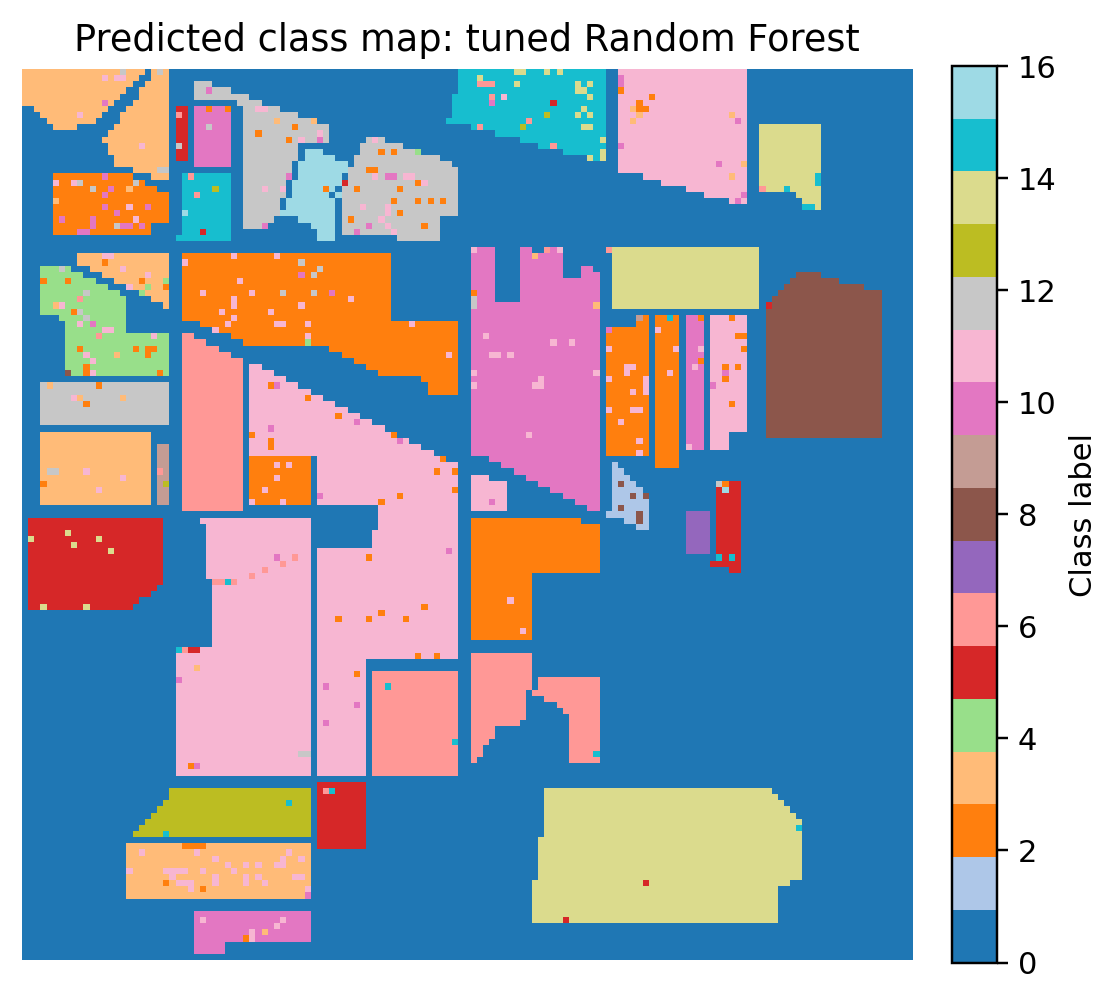
\includegraphics[width=0.62\textwidth]{outputs/figures/11_prediction_map.png}
\caption{Spatial prediction map generated using the tuned Random Forest.}
\end{figure}

\section{Discussion}

\subsection{Why SVM Performed Best}

SVM likely performed best because the dataset has high-dimensional spectral information, and SVM is known to work well in high-dimensional spaces. After median imputation, standardization, and PCA, the transformed features are more compact and less noisy. The RBF kernel then allows SVM to learn nonlinear boundaries between classes.

\subsection{Interpretation of Cleaning Decisions}

The missing-value and infinite-value checks showed that the corrected cube is numerically complete. For this reason, no row deletion or actual value replacement was necessary. Median imputation was still kept in the pipeline because it documents the filling method and makes the workflow robust if future data contain missing values.

The IQR rule flagged unusual spectral values, but those values were retained. This is justified because hyperspectral outliers can be valid material signatures. Removing them automatically could also reduce the already-small minority classes and make the classifier less fair.

\subsection{Interpretation of Encoding and Embedding}

One-hot encoding was not used for the input data because the features are continuous spectral measurements. Applying one-hot encoding to continuous bands would destroy the numerical meaning of reflectance values. PCA is the correct embedding method for this project because it keeps the numerical structure while reducing the 200-band representation to 20 informative components.

\subsection{Effect of Class Imbalance}

Class imbalance remains one of the main limitations. Classes with very few samples, such as Oats and Grass-pasture-mowed, are difficult for models to learn. Even if the overall accuracy is high, minority classes may still have weaker recall.

\subsection{Importance of PCA}

PCA helped simplify the problem by reducing 200 bands to 20 principal components while preserving approximately 97.64\% of the standardized spectral variance. This is important because using all original bands could increase computation time and include redundant information. PCA also helps visualize how much variance is preserved as dimensionality increases.

\section{Limitations}

This project has some limitations:

\begin{itemize}
    \item The dataset is imbalanced, which affects minority-class performance.
    \item The model treats each pixel independently and does not use spatial neighborhood information.
    \item Only a limited hyperparameter search was performed to keep the project computationally practical.
    \item Deep learning models were not tested.
    \item PCA components are less directly interpretable than original spectral bands.
    \item IQR flags were analyzed diagnostically, but no manual field validation was available to confirm whether flagged pixels were sensor noise or valid rare spectra.
\end{itemize}

\section{Future Improvements}

Future work could improve the project in several ways:

\begin{itemize}
    \item Use spatial features from neighboring pixels.
    \item Try convolutional neural networks for spatial-spectral classification.
    \item Apply class balancing techniques such as oversampling or class-weight tuning.
    \item Perform a larger hyperparameter search.
    \item Compare PCA with other dimensionality reduction methods such as Linear Discriminant Analysis or autoencoders.
    \item Evaluate per-class precision and recall more deeply for minority classes.
    \item Compare IQR retention with robust scaling or winsorization in a controlled experiment.
\end{itemize}

\section{Conclusion}

This project successfully applies a complete data mining workflow to the Indian Pines hyperspectral imaging dataset. The selected task is multi-class classification, where each labeled pixel is classified into one of 16 land-cover categories.

The data collection and visualization stage loaded the corrected hyperspectral cube, displayed the pseudo-RGB image and ground-truth map, and analyzed class distribution, spectral signatures, and band correlation. The cleaning stage removed unlabeled pixels, reshaped the image into a feature matrix, checked missing values, checked infinite values, checked duplicate rows, and applied IQR diagnostics. A band-and-pixel cleaning visualization was added to connect the IQR flags back to the spatial image and a real spectral signature. IQR-flagged pixels were preserved because they may be valid spectral signatures and because minority classes are already small.

The preprocessing design included median imputation, standardization, PCA embedding, stratified train-test splitting, baseline models, three main classifiers, cross-validation, and hyperparameter tuning. One-hot encoding was not applied because the input features are continuous spectral bands. The Most Common Class baseline achieved only 23.95\% accuracy, while k-Nearest Neighbors achieved 74.88\%. Among the main models, Support Vector Machine performed best with 81.17\% test accuracy, 80.45\% cross-validation accuracy, 84.03\% macro F1-score, and 81.26\% weighted F1-score.

Overall, the results show that hyperspectral image classification benefits from careful preprocessing, dimensionality reduction, and suitable classifier selection. SVM is the best model in this experiment, while class imbalance remains the main challenge for future improvement.

\newpage
\appendix

\section{Reproducibility Notes}

The project was implemented in a Jupyter notebook using NumPy, pandas, matplotlib, SciPy, and scikit-learn. The notebook is the single runnable codebase for the project. The same random seed was used throughout the experiment:

\begin{itemize}
    \item Random seed: 42.
    \item Test size: 20\%.
    \item PCA components: 20.
    \item Cross-validation: 3-fold stratified.
    \item Missing-value filling method: median imputation inside each pipeline.
    \item Feature encoding decision: no one-hot encoding for continuous spectral bands.
\end{itemize}

\section{Core Modeling Pipeline}

The main machine learning workflow can be summarized as:

\begin{verbatim}
Pipeline([
    ("imputer", SimpleImputer(strategy="median")),
    ("scaler", StandardScaler()),
    ("pca", PCA(n_components=20, random_state=42)),
    ("model", Classifier())
])
\end{verbatim}

This pipeline was used to avoid data leakage and to ensure that preprocessing was applied consistently during training, testing, cross-validation, and tuning.

\section{Notebook and Report Alignment}

The Jupyter notebook and this report use the same main experimental settings:

\begin{itemize}
    \item Same dataset files: \texttt{Indian\_pines\_corrected.mat} and \texttt{Indian\_pines\_gt.mat}.
    \item Same problem type: multi-class classification.
    \item Same number of PCA components: 20.
    \item Same filling method: median imputation inside each modeling pipeline.
    \item Same encoding decision: no feature one-hot encoding because all predictors are numerical spectral bands.
    \item Same train-test split: 80\% training and 20\% testing with stratification.
    \item Same random seed: 42.
    \item Same cleaning-diagnostic figure: band 40 and the selected high-flag class-15 pixel.
    \item Same baseline models: Most Common Class and k-Nearest Neighbors.
    \item Same main models: Random Forest, Gradient Boosting, and Support Vector Machine.
    \item Same cross-validation strategy: 3-fold stratified cross-validation.
    \item Same Random Forest tuning methods: RandomizedSearchCV and GridSearchCV.
\end{itemize}

\end{document}
